\documentclass[11pt,a4paper,parskip]{scrartcl}
%\def\xcolorversion{2.00}
%\def\xkeyvalversion{1.8}
\usepackage[utf8x]{inputenc}
%\usepackage{ucs}
\usepackage{amsmath}
\usepackage{amsfonts}
\usepackage{amssymb}
\usepackage{graphicx}
\usepackage{lmodern}
\usepackage{hyperref}
\usepackage[ngerman]{babel}
\usepackage{pdfpages}
%\usepackage[version=0.96]{pgf}
%Tikz Beginn
    \usepackage{tikz} 
    \usepackage{pgfplots}
%Tikz Ende
%Glossar, Abkürzungsverzeichnis Beginn
    \usepackage[acronym]{glossaries} %Glossar %\usepackage[acronym, toc]{glossaries} %Glossar mit Aufruf im Inhaltsverzeichnis
    \makeglossaries
    \newglossaryentry{Ablaufberg}{
    name=Ablaufberg,
    description={Der Ablaufberg ist ein in der Regel künstlich angelegter Hügel, über den ein Gleis verläuft. Ablaufberge dienen beim Abdrücken dem Ablaufen lassen von Güter- wagen, die auf diese Weise nach ihren Bestimmungsorten sortiert werden}
}
%	Bedienfahrt	
%	Bezetteln   
\newglossaryentry{Bremsprobe}{
    name=Bremsprobe,
    description={Eine Bremsprobe  ist ein zur Vorbereitung von Zugfahrten gehörender Vorgang, bei dem die Funktionsfähigkeit des Bremssystems der Fahrzeuge im Zugverband überprüft wird. Dabei wird im Stillstand das Anlegen und Lösen der zu prüfenden Bremsen kontrolliert%. Siehe dazu auch Anhang \ref{sec:ABremsen}
    }
}
\newglossaryentry{Eisenbahnverkehrsunternehmen}{
    name=Eisenbahnverkehrsunternehmen,
    description={Eisenbahnverkehrsunternehmen sind Eisenbahnen, die Eisenbahnverkehrsleistungen erbringen. \acrshort{EVU}s müssen in der Lage sein, die Zugförderung (Traktion) sicherzustellen\cite{rennsteigbahn}}
}
\newglossaryentry{Heisslaeuferortungsanlage}{
    name=Hei\ss l\" auferortungsanlage,
    description={Eine Heißläuferortungsanlage dient dazu, eine unzulässige Er- wärmung von Radsatzlagern durch Defekte bei Schienenfahrzeugen (sogenannte Heiß- läufer) rechtzeitig feststellen zu können}
}
\newglossaryentry{ep-Bremse}{
    name=ep-Bremse,
    description={Die elektropneumatische Bremse (ep-Bremse) ist eine durch elektropneumatische Bauteile gesteuerte automatische Druckluftbremse bei Eisenbahnen. Die ep-Bremse ermöglicht das gleichzeitige Bremsen oder Lösen aller Fahrzeuge unabhängig von der Länge des Zuges}
}
\newglossaryentry{ep-''light''-Bremse}{
    name=ep-''light''-Bremse,
    description={Was genau macht sie jetzt?
    }
}
\newglossaryentry{EOW}{
    name=EOW,
    description={Eine elektrisch ortsgestellte Weiche (EOW) ist eine elektrisch angetriebene Weiche, die nicht von einem Stellwerk, sondern vom Weichenort aus direkt bedient wird. EOW sind das moderne Äquivalent zu Handweichen und werden hauptsächlich in Gleisanlagen eingesetzt, in denen nur frei rangiert wird}
}
\newglossaryentry{Bergbremse}{
    name=Bergbremse,
    description={Bergbremsen sorgen bei großen Rangierbahnhöfen nach erfolgter Geschwindigkeitsmessung für eine Vorabbremsung, damit die Talbremsen ihre Funktion erfüllen können}
    }
\newglossaryentry{Talbremse}{
    name=Talbremse,
    description={Talbremsen verzögern Wagen vor einer Richtungsgleisgruppe, so dass der Abstand zum vorherlaufenden Wagen groß genug bleibt, damit die Weichen in der Lücke umgestellt werden können}
    }
\newglossaryentry{Gleisanschluss}{
    name=Gleisanschluss,
    description={Ein Gleisanschluss ist ein Schienenweg zur Erschließung eines Geländes oder Gebäudes, das selbst nicht zur öffentlichen Eisenbahninfrastruktur gehört}
}
\newglossaryentry{Hemmschuh}{
    name=Hemmschuh,
    description={Ein Hemmschuh ist eine keilförmige Konstruktion zum Festhalten von Schienenfahrzeugen. Er wird zwischen Rad und Schiene platziert, um durch die entstehende Reibung den Wagen zu bremsen beziehungswies an (selbstständiger) Bewegung zu hindern}
}
\newglossaryentry{Knotenbahnhof}{
    name=Knotenbahnhof,
    description={Ein Knotenbahnhof ist eine Bahnhof der für Betriebsabläufe zur Zugbereitstellung oder Verknüpfung mit anderen Verkehrsträgern erforderlich ist}
}
\newglossaryentry{Rangierbahnhof}{
    name=Rangierbahnhof,
    description={Rangierbahnhöfe sind die Zugbildungsbahnhöfe des Einzelwagenverkehrs im Güterverkehr der Eisenbahn}
}
\newglossaryentry{Rangierfahrt}{
    name=Rangierfahrt,
    description={Rangierfahrten bezeichnen das Bewegen einzelner Schienenfahrzeuge oder Fahrzeuggruppen, soweit es sich nicht um eine Zugfahrt (einschließlich Sperrfahrt) handelt}
}
%\newglossaryentry{Rangiermittel}{
 %   name=Rangiermittel,
  %  description={Rangiermittel sind Ein- oder Zweiwegefahrzeuge die (mit Elektroantrieb und oder im Handbetrieb) Die Aufgaben von Rangierlokomotiven übernehmen.}
%}
\newglossaryentry{Satellitenbahnhof}{
    name=Satellitenbahnhof,
    description={Satellitenbahnhöfe bestehen in der Regel aus kleinen Gleisanlagen ohne Rangiereinrichtungen und -personal. Sie dienen der Sammlung und Verteilung Güterwagen auf die Lokalen Gleisanschlüsse\cite{Verkehrslogistik}}
}
%\newglossaryentry{Sägefahrten}{
 %   name=Sägefahrten,
  %  description={Sägefahrten sind das koordinierte Vor- und Zurücksetzen von Wagen zum rangieren von Wagen.}
%}
\newglossaryentry{Schiebewandwagen}{
    name=Schiebewandwagen,
    description={Der gedeckte Güterwagen der Sonderbauart H, oder auch Schiebewandwagen, ist ein gebräuchlicher Wagen für nässeempfindliche, pallettierte Ware. Die verschieblichen Seitenwände ermöglichen es, die ganze Ladefläche von der Seite her zu be- und entladen}
}
\newglossaryentry{Sperrfahrt}{
    name=Sperrfahrt,
    description={Sperrfahrten sind Fahrten, die in ein Gleis der freien Strecke eingelassen werden, das gesperrt ist. Dies dient der Bedienung einer Anschlussstelle auf der freien Strecke\cite{RIL408}}
}
\newglossaryentry{Zugfahrt}{
    name=Zugfahrt,
    description={Eine Zugfahrt bezeichnet eine Fahrt im Bahnhof und auf der Strecke, die durch Hauptsignale gesichert und geregelt ist, sowie Züge im Bereich mit Führerstandsignali- sierung. Bei dieser Fahrt ist der Fahrweg bis zum Ende frei. Es wird Flankenschutz gewährt und Weichen gegen Umstellen gesichert. Die Strecke für die Zugfahrt hat eine maximale Geschwindigkeit vorgegeben, der Zug hat eine feste Zusammensetzung und eine eindeutige Zugnummer für diese Fahrt}
}
\newglossaryentry{Zugschluss}{
    name=Zugschluss,
    description={	Der Zugschluss bezeichnet den letzten Wagen eines Zuges. Dieser ist vom Zugschlusssignal gekennzeichent. Mit seiner Hilfe kann die Vollständigkeit von Zügen, visuell durch das Personal des Bahnbetriebs, überprüft werden}
}
\newglossaryentry{Vorbahnhof}{
    name=Vorbahnhof,
    description={Als Vorbahnhof bezeichnet man den äußeren Teil eines großen Bahnhofes oder auch einen Bahnhof in der Nähe eines großen Bahnhofs, der diesem Aufgaben abnimmt}
}
\newglossaryentry{Lokrangierfuehrer}{
    name=Lokrangierf\"uhrer,
    description={Der Lokrangierführer ist eine Bezeichnung für einen Triebfahrzeug- führer oder einen Eisenbahnfahrzeugführer von Lokomotiven mit Funkfernsteuerung im Rangierdienst}
}
\newglossaryentry{Eisenbahnbetriebsleiter}{
    name=Eisenbahnbetriebsleiter,
    description={Eisenbahnbetriebsleiter leiten und überwachen die sicherheitsrelevanten Abläufe in einem Eisenbahnunternehmen, das keinen grenzüberschreitenden Verkehr aufweist}
}
\newglossaryentry{Bremsprobeberechtigte}{
    name=Bremsprobeberechtigte,
    description={Der Bremsprobeberechtigte ist ein für die Bremsprobe ausgebildeter Mitarbeiter, der die Bremsprobe durchführen darf. Häufig haben Triebfahrtzeugführer diese Zusatzausbildung selbst, um die Bremsprobe selbstständig durchführen zu können}
}
\newglossaryentry{Bremsprobeanlage}{
    name=Bremsprobeanlage,
    description={Eine Bremsprobeanlage wird für die Herstellung der Betriebsbereitschaft eines Eisenbahnzuges benötigt. Sie dient dazu eine Hauptbremsprobe am Zugverband durchzuführen. Diese Hauptbremsprobe kann zwar auch ohne eine entsprechende (ortsfeste) Anlage durchgeführt werden, dann muss aber ein Triebfahrzeug und ein weiterer Bremsprobeberechntigter vorhanden sein. Aus Kostengründen werden deshalb in größeren Formationsbahnhöfen ortsfeste Bremsprobeanlagen eingesetzt, da damit Triebfahrzeuge und Personal eingespart werden können}
}

\newglossaryentry{konventioneller Gueterwagen}{
    name=konventioneller G\"uterwagen,
    description={Als konventionelle Güterwagen werden die Güterwagen bezeichnet, die aus konventionellen (herkömmlichen) Komponenten, wie Drehgestellen, Kupplungen, Bremsen und Wagenkästen, bestehen}
}

\newglossaryentry{Gueterwagen 40}{
    name=G\"uterwagen 4.0,
    description={Als Güterwagen 4.0 wird der vollständig ausgebaute Güterwagen bezeichnet}
}

\newglossaryentry{Demonstrator}{
    name=Demonstrator,
    description={Als Demonstrator wird der in diesem Projekt modifizierte Güterwagen bezeichnet. Er stellt eine Teilmenge des Güterwagen 4.0 dar}
}

\newglossaryentry{40-Komponenten}{
    name=4.0-Komponenten,
    description={4.0-Komponenten sind die Subsysteme, die den konventionellen Güter- wagen zu einem Güterwagen 4.0 machen. Zu diesen Komponenten gehören die Energieversorgung, Aktoren und Sensoren sowie die Kommunikationssysteme des Güterwagen}
}

\newglossaryentry{Wagenzug}{
    name=Wagenzug,
    description={Ein Wagenzug ist ein gekuppelter Verband nicht angetriebenen Güterwagen}
}

\newglossaryentry{Zugverband}{
    name=Zugverband,
    description={Ein Verbund aus Güterwagen und Lok wird als Zugverband bezeichnet}
}

\newglossaryentry{Lastwechsel}{
    name=Lastwechsel,
    description={Die Ausstattung mit Lastwechsel ermöglicht das Anpassen des Bremsklotzdrucks an das effektive Wagengewicht. Sie verhindert ein Überbremsen bei geringer Zuladung und wirkt zu schwacher Bremskraft bei beladenen Fahrzeugen entgegen. Wenn bei gleichbleibender Bremskraft das Fahrzeuggewicht durch die Beladung zunimmt, verringert sich die Bremswirkung. Darum ist die Umstelleinrichtung in die passende Stellung („leer“, „beladen“ oder ggf. „teilbeladen“) manuell oder automatisch zu bringen}
}
    %\newacronym{AK}{AK}{Automatikkuppung}
\newacronym{DIN}{DIN}{Deutsches Institut für Normung}
%\newacronym{EOW}{EOW}{Elektisch ortsgestellte Weiche}
\newacronym{EN}{EN}{Europäische Normung}
\newacronym{EVU}{EVU}{Eisenbahnverkehrsunternehmen}
%\newacronym{FHAC}{FH Aachen}{Fachhochschule Aachen, University of applied Science}
\newacronym{HL}{HL}{Hauptluftleitung}
%\newacronym{ISO}{ISO}{International Organisation for Standardisation	(dt.: Internationale Organisation für Normung)}
\newacronym{RIL}{RIL}{Richtlinie}
\newacronym{twb}{TWb}{Technische Wagenbehandlung}
%Glossar, Abkürzungsverzeichnis Ende
\usepackage{verbatim}
%Quellen Beginn
    \usepackage[backend=bibtex,
        style=numeric,
        bibencoding=ascii
        %style=alphabetic
        %style=reading
    ]{biblatex}
    \addbibresource{Kapitel/Quellen.bib}
%Quellen Ende
%Anforderungsnummerierung nach Raphael Beginn
    %\theoremstyle{remark}
    \newtheorem{rem}{Notiz}
    %\theoremstyle{definition}
    \newtheorem{feat}{Merkmal}
    %\newtheoremstyle{definition}% name of the style to be used
    %  {5pt}% measure of space to leave above the theorem. E.g.: 3pt
    %  {5pt}% measure of space to leave below the theorem. E.g.: 3pt
    %  {}% name of font to use in the body of the theorem
    %  {}% measure of space to indent
    %  {\bfseries}% name of head font
    %  {}% punctuation between head and body
    %  {\newline}% space after theorem head; " " = normal interword space
    %  {}% Manually specify head
%Anforderungsnummerierung nach Raphael Ende

%zugehörige Dokumente
    \newtheorem{dok}{Dokument}

\begin{document} 
\setlength{\parskip}{5mm}% plus5mm minus5mm} %Absatzlänge

%Deckblatt Beginn
    \begin{titlepage}
        \newcommand{\HRule}{\rule{\linewidth}{0.5mm}} % Defines a new command for the horizontal lines, change thickness here
        \center % Center everything on the page
        \vspace*{2cm}
        \textsc{\LARGE Neue Elektronik- und Kommunikationssysteme für den intelligenten, vernetzten Güterwagen}\\[1.5cm] % Name of your university/college
        %    \textsc{\Large Neue Elektronik- und Kommunikationssysteme für den intelligenten, vernetzten Güterwagen}\\[0.5cm] % Major heading such as course name
        \textsc{\large FKZ 16ES0850K}\\[0.5cm] % Minor heading such as course title
        \HRule \\[0.4cm]
        { \huge \bfseries Lastenheft}\\[0.4cm] % Title of your document
        \HRule \\[1.5cm]
        \begin{minipage}{0.4\textwidth}
        \begin{flushleft} \large
        \emph{FH Aachen}\\
        Daniela \textsc{Wilbring}\\
        Prof. Dr.-Ing. Manfred \textsc{Enning},\\
        Prof. Dr.-Ing. Bernd \textsc{Schmidt},\\
        Prof. Dr. Raphael \textsc{Pfaff}\\
        \end{flushleft}
        \end{minipage}
        ~
        \begin{minipage}{0.4\textwidth}
        \begin{flushright} \large
        \end{flushright}
        \end{minipage}\\[2cm]
        {\large \today}\\[2cm] % Date, change the \today to a set date if you want to be precise
        \vfill % Fill the rest of the page with whitespace
    \end{titlepage}
%Deckblattt Ende

\pagenumbering{roman}
\section*{Zweck des Dokuments}
Das Lastenheft ist, nach DIN 69901-5\footnote{Projektmanagement – Projektmanagementsysteme – Teil 5: Begriffe}, ''die vom Auftraggeber festgelegte Gesamtheit der Forderungen an die Lieferungen und Leistungen eines Auftragnehmers innerhalb eines (Projekt-)Auftrags''.\par
Ein Lastenheft ist wichtig in der Analysephase und zur Kommunikation innerhalb des Auftrages/Projekts. Es bietet eine ausführliche Beschreibung der Arbeitsleistung und dient als Kommunikationsbasis.\par
Auf Basis des Lastenheftes wird das Pflichtenheft vom Auftragnehmer erarbeitet.\par
Untersuchungen zeigen, dass Fehler in der Produktentwicklung bei einer späten Aufdeckung und Behebung teurer werden als bei einer früheren Erkennung. Deshalb sollte man schon beim Lastenheft eine hohe Qualität anstreben.\footnote{Quelle: \url{https://www.pm-blog.eu/themen/methoden/lastenhefte-eine-schrittweise-anleitung-fur-den-perfekten-aufbau.html} }\par
In diesem Fall wird das Lastenheft im Rahmen des Projektes "Neue Elektronik- und Kommunikationssysteme für den intelligenten, vernetzten Güterwagen" von der FH Aachen als Vorarbeit für das Pflichtenheft erstellt. \par
Klare gemeinsame Ziele innerhalb des Projektes sollen zu einer besseren und strukturierten Zusammenarbeit führen.
%Das Lastenheft wird aufgrund von Veröffentlichungen der Projektsteller und dem Gesamtverbundantrag des Projektes erstellt

%Verzeichnisse Beginn
    \section*{Revisionshistorie}
\begin{tabular}{|p{3cm}|p{2cm}|p{5.5cm}|p{2cm}|}
\hline
Versionsnummer  & Datum         & Beschreibung          & Autor     \\
\hline
 1.0.0          & 28.02.2019    & Erstellung Lastenheft & Wilbring  \\\hline
                &               &                       &           \\\hline
\end{tabular}

% Aufbau Versionsnummmer
% 1.2.3
    % 1 - Hauptversionsnummer - Signifikante Änderung am Lastenheft - Änderungnen Inhaltsverzeichnis, Strukturänderung, ...
    % 2 - Nebenversionsnummer - Funktionale Änderung am Lastenheft - weitere Anforderungen, Ausführungen in Unterkapiteln, ...
    % 3 - Revisionsnummer - Kleine Änderungen am Lastenheft - Fehlerbehebung, Orthographie, ...\newpage
    \tableofcontents \newpage
    \listoffigures %\addcontentsline{toc}{section}{Abbildungsverzeichnis}
    %\listoftables %Tabellenverzeichnis 
    \printglossary[title= Abkürzungen, 
        %toctitle=Abkürzungen, 
        type=\acronymtype]
    \printglossary\newpage
%Verzeichnisse Ende

%Hauptteil Beginn
\pagenumbering{arabic}
    \section{Einleitung}
Der Güterverkehr in Deutschland wird bislang zu über 70\% von LKWs gestemmt, was Verkehrsstaus und hohe Schadstoffemissionen verursacht. Das Zukunftsprojekt Industrie 4.0 bietet dem Schienengüterverkehr die einzigartige Chance, durch intelligente Steuerung und Vernetzung Transportprozesse extrem flexibel, effizient und schadstoffarm zu gestalten. Realisiert werden kann dies durch die Integration vielfältiger moderner Sensorik und Elektronik in den Güterwagen4.0.\footnote{Antrag auf Gewährung einer Bundeszuwendung auf Ausgabenbasis (AZAP), 26.04.2018}\par
%Im Projekt werden Sensoren und Elektroniksysteme zur Realisierung eines „intelligenten“, mittels Industrie 4.0-Technologien vernetzten Güterwagens entwickelt. Die Sensorik dient dabei der Online-Erfassung relevanter Güterwagen- und Zugverbund-Daten zur Zustands- und Verschleißanalyse. Durch diese Informationen wird erstmals eine durchgängige Logistik und die von Kunden geforderte Transparenz der Lieferkette sowie eine vorausschauende Planung von Wartungszyklen und Rentabilität für den Güterwagenbetreiber ermöglicht. Als weiterer Lösungsansatz werden Aktoren entwickelt und in den Güterwagen4.0 integriert, mit denen die beim Zusammenstellen bzw. Trennen von Güterwagen erforderlichen aufwendigen und oft sicherheitsrelevanten manuellen Tätigkeiten künftig vollautomatisiert durchgeführt und sensorisch online überwacht werden können.\footnote{Antrag auf Gewährung einer Bundeszuwendung auf Ausgabenbasis (AZAP), 26.04.2018}\\
%Der Güterwagen4.0 stellt einen wichtigen Baustein zur Lösung der gravierenden Verkehrsprobleme dar. Die Ergebnisse des Vorhabens tragen wesentlich dazu bei, durch einen zukunftsfähigen Schienenverkehr Verkehrsstaus und Schadstoffemissionen zu vermindern. Die angestrebten sensorischen Fähigkeiten des Güterwagen4.0 erlauben perspektivisch auch eine Übertragung in den Schienenpersonenverkehr.\footnote{Antrag auf Gewährung einer Bundeszuwendung auf Ausgabenbasis (AZAP), 26.04.2018}\\\\
In diesem Lastenheft wird anhand eines Schiebewandwagens der grobe Ablauf eines Umlaufs im bisherigen System erläutert und daraufhin Anforderungen an den neuen Güterwagen erstellt. Als Motivation zeigen sich %neben der oben bereits erwähnten Verringerung von Verkehrsstaus und Schadstoffemissionen auch 
eine Erhöhung der Prozesssicherheit, Verringerung der aufzuwendenden Zeit am Wagen, eine Gestaltung von attraktiveren Arbeitsplätzen durch eine ergonomischere Arbeitsgestaltung und mögliche Kosteneinsparungen an der Infrastruktur.\par
Herausforderungen wie die Migration und Annahme des Systems sollen beachtet werden. Die Kosten des Systems, sowie dessen Einbau müssen konkretisiert werden. Prozesse für produktivere Arbeitsabläufe mit dem neuen Güterwagen müssen gestaltet werden. Arbeitsabläufe bei Defekten konkretisiert werden.\\

Hier fehlt eine Erklärung wo die Reise hin gehen soll, ein Fokus, was wir uns vom GW40 erhoffen und eine sensibilisierung für den Prozess und das Vorgehen zur Änderung dessen.\\
Es ist geplant eine Möglichkeit für produktivere Verkehre zu schaffen.\\
Automatisierungslösungenen  Automatisches Abdrücken mit AK o. automatischer Schraubenkupplung – Trennstellen, Kommunikation mit Bergrechner – Vorbereitung Ablauf\\
• Vorteile des Systems\\
Dezentralität\\
Zukunftssicher\\
muss nicht auf AK warten, funktioniert aber auch damit\\
Wertschöpfungsprozess\\
Automatisierung\\
Automatisierung Bremse – Bremse lösen, lüften, Handbremse, Berechnung Bremsgewichte, Durchgängigkeit HL, automatische Bremsprobe, automatischer Bremszettel\\
Vorbereitung Trennstellen – HL-Absperrhähne Schließen, lüften, 2x Signal = trennen – Signal: kann, soll trennen \newpage
    \section{Ist-Zustand}\label{sec:Istzustand} %Beschreibung wo Produktivität vergudet wird um daraus ableiten zu können, was benötigt wird. % Kochsiek, Knoll nach Meinung zu diesem Kapitel fragen!
Im Folgenden wir der Umlauf eines \gls{Schiebewandwagen} (Habinns) beschrieben. Der Wagen wird in einem \gls{Gleisanschluss}/RailPort mit palletiertem Gut beladen, läuft dann durch das deutsche/europäische Einzelwagensystem und wird in einer Ladestelle an einem Gleisanschluss oder RailPort entladen. Fokus dieser Beschreibung sind die durchzuführenden manuellen Tätigkeiten. Davon leitet sich im Folgenden ein Anforderungskatalog an einen aktiven, kommunikativen Güterwagen 4.0 ab, der viele oder alle der manuellen Tätigkeiten durch Technikfunktionen ersetzt.
Die hier beschriebenen Prozesse sind leicht idealisiert. So werden Störfälle erst einmal ausgenommen. Auch kann davon ausgegangen werden, dass jede Prozess leicht anders aussieht. Trotzdem zeigt er viele wichtige Punkte, die verbessert werden können und sollten. Bei anderen Wagenarten unterscheidet sich der Umlauf natürlich noch weiter. Weitere Informationen zu anderen Prozessen und vor allem auch zu Prozessen in der Disposition sind im Anhang \ref{sec:realeIst} zu finden. \par
\subsection{Vorgänge an der Ladestelle/im Gleisanschluss}
%In diesem Unterkapitel wird eine kurze Beschreibung def Fahrwege, Bewegung von Fahrzeugen, der Personaltätigkeit sowie der Beladung, dem Wagenwechsel, der Ladungsicherung und der benötigten Transportdokumente gegeben.
\subsubsection{Fahrweg} \label{sec:Fahrweg}
Die Bewegung von Wagen erfolgt prinzipiell auf Gleisen. Eine Verzweigung von Fahrwegen erfordert Weichen. In kleinen und mittleren Gleisanschlüssen sind dies überwiegend handbetätigte Weichen. 
\subsubsection{Bewegung der Wagen} \label{sec:BewdWagen}
Je nach Wagenaufkommen kommen folgende Methoden der Wagenbewegung in Betracht:
\begin{itemize}
	\item Bedienung durch das \acrshort{EVU}, welches auch die Zustellfahrten durchführt
	\item Eigene (zum \gls{Gleisanschluss} zugehörige) Rangierlokomotive
	\item Eigenes Rangierhilfsmittel
	\begin{itemize}
	    \item Gleisfahrbar (Rangierroboter)
	    \item Zweiwegefahrzeug
	\end{itemize}
	\item Stationäre Verschubeinrichtung (Seilzuganlage)
	\item Verschub mittels Muskelkraft von Tieren oder Menschen (z.B. Knippstange, Wagenrücker)
\end{itemize}
\subsubsection{Personalfähigkeiten}\label{sec:Personal}
Allen Methoden ist gemeinsam, dass Sie spezielle Personalfähigkeiten bzw. eine entsprechende Ausbildung benötigen. Dies ist nicht zuletzt auf die Tatsache zurückzuführen, dass ein einmal in Bewegung gesetzter Güterwagen auch bei langsamer Fahrt eine hohe kinetische Energie aufweist. Zusätzlich ist die Bedienung der Wagenbremsen (Luft- und/oder Handbremse) für ungeschultes Personal kompliziert und fehleranfällig.
\subsubsection{Bereitstellung}
Eine Bereitstellung der Wagen findet aus einem \gls{Vorbahnhof} als Einfahrgruppe oder Ordnungsgruppe statt. Diese stehen dort im Allgemeinen mit entlüfteter Bremse und vorgelegtem Hemmschuh oder angelegter Handbremse.
\subsubsection{Beladung}
Das Beladen von Güterwagen mit Paletten erfolgt von einer Rampe oder einer Ladekante mit Überfahrbrücke aus in der Regel per Gabelstapler. Im Gegensatz zur Heckbeladung von LKW existieren kaum Lösungen zur Automatisierung der Beladung. Dies ist ein Logistikprozess des Verladers.
\subsubsection{Ladungssicherung}
Während oder nach der Beladung muss die Ladung gegen Verrutschen gesichert werden. Bei Schiebewandwagen erfolgt dies unter anderem durch von Hand verschiebbare und durch Verriegeln zu sichernde Zwischenwände. Auch für diese Aufgabe ist der Verlader verantwortlich. Er muss den Wagen als bahntechnisch sicher an das EVU übergeben. Das EVU darf nur mit einem augenscheinlich (also für den Beobachter sicheren) Wagen fahren. Dies betrifft in einem geschlossenen Wagen nicht die Ladung, aber die Türen und Verschlüsse; auf einem offenen (Holz-)Transporter aber auch die sichtbare Ladung. Bei Gefahrgut müssen noch weitere Kontrollen von geschultem Personal durchgeführt und der Wagen passend gekennzeichnet werden.
\subsubsection{Wagenwechsel}
Eine Ladekante ist meist für Einzelwagen oder kleine Gruppen (bis max. ca. 4 Wagen) gestaltet, so dass häufig Wagen an der Ladestelle getauscht werden müssen, bevor die Zustellfahrt erfolgt. Dies liegt unteranderem an der Seitenbeladung, für die viel Platz benötigt wird. Diese hat, gegenüber der Heckbeladung bei LKW, den Vorteil der Parallelisierbarkeit. LKW gehen nach der Beladung direkt in den Umlauf, sodass bei diesen das häufige Umsetzen nicht als Nachteil gesehen wird. \par
Beim Beladen von Wagen mit Gefahrgut, ist es üblich die Weichen vor und hinter der Beladestelle in der dem Beladegleis abgewandten Position abzuschließen. Dies soll ein ungewolltes Bewegen der Wagen verhindern. Diese Weichen werden vom Verlader erst nach Beenden der Verladearbeiten wieder geöffnet.\par
Wagen können grundsätzlich rangiert oder verschoben werden. Findet die Wagenbewegung mit \gls{Lokrangierfuehrer} (\acrshort{LRF}) und Lok statt, wird rangiert. Verschoben werden die Wagen wenn die Wagenbewegung ohne Lok und Lokrangierführer stattfindet.\par
Rangiert wird wenn möglich ohne Luftkupplung und entsprechend auch ohne \gls{Bremsprobe}. Ob Rangieren ohne Luftkupplung möglich ist, hängt von der Lokomotive, der Last, der Achsenanzahl der zu rangierenden Wagen und der Neigung des Ladegleises ab. Muss aufgrund dieser Eigenschaften mit Luft gefahren werden, ist auch eine vereinfachte \gls{Bremsprobe} notwendig. Häufig findet diese Rangierfahrt in der Bremsstellung G statt.\par
Im Allgemeinen werden einzelene Wagen oder kleinere Wagengruppen für nur wenige Meter verschoben. Dies kann zum Beispiel mit einem Zwei-Wege-Fahrzeug auf LKW-Basis stattfinden. Hier verschiebt ein angelernter und unterwiesener Verlademitarbeiter mit einem zusätzlichen Sicherheitsposten die Wagen. Der Verlademitarbeiter wird vom \gls{Eisenbahnbetriebsleiter} (\acrshort{EBL}) angelernt und unterwiesen.
\subsubsection{Transportdokumente}\label{sec:Transdoc}
Im LKW-Bereich entstehen bereits Lösungen zur papierlosen Transportabwicklung einschließlich der Behandlung von Gefahrgutdokumenten. Bei Bahntransporten herrscht die klassische Methode der Übergabe von Frachtdokumenten an das \acrshort{EVU} vor. Oft werden diese auch direkt elektronisch übergeben. Dann sind diese später digital verfügbar. Ausgenommen sind Gefahrgutscheine, diese werden immer als Papierzettel mitgeführt. Auch die Wagen werden, vorallem im Einzelwagenverkehr noch "`bezettelt"'\footnote{Siehe dazu auch VDV-Schrift 758 - Prüfen von Güterwagen im Eisenbahnbetrieb}. Diese Zettel sind Vereinfachungen des Frachtbriefes, die direkt auf dem Wagen mitgeführt werden. Auf diesen steht im Allgemeinen aus was die Ladung besteht, woher diese kommt und wohin sie geht. Auch weitere Besonderheiten werden hier vermerkt.
%Der Lkw wird meist in Längsrichtung durch das Heck an einem Tor / Vorsatzschleuse beladen. Für die eigentliche Beladung ist es  ungünstiger als die Seitenbeladung, es führt aber zu einer effizienten Flächennutzung in der Halle (Zeilenstruktur). Daher ist die Heckbeladung gerade bei Logistik/Verteilzentren und Speditionen heute die vorherrschende Methode.  
%Für spezielle Güter / Wagen ist Beladung mit Hallenkran von oben üblich (Papier, Stahlcoils)
\subsection{Abholen im Gleisanschluss}
Die Abholung von Wagen erfolgt entweder durch das \acrshort{EVU} unmittelbar an der Ladestelle oder -- wenn lokale Rangierhilfsmittel zur Verfügung stehen -- von einem Übergabegleis im Werksgelände. Die Bedienung des Anschlusses ist in der Regel Teil eines Umlaufs, in dem mehrere Anschlüsse nacheinander bedient werden.
\subsubsection{Luft- und mechanische Kupplung}\label{sec:LuftumechKup}
Der oder die Wagen stehen im festgelegten Zustand zur Abholung bereit. Die Luftbremse ist gewöhnlich außer Funktion, der Reserveluftbehälter ist leer. Nach dem Ansetzen der Lok bzw. des aktuell letzten Wagens der Rangierabteilung ist manuell zu kuppeln. Der Lokführer oder Rangierbegleiter "`taucht"' dazu unter den Puffern durch und verbindet zunächst manuell die Schraubenkupplung. Danach wird die Hauptluftleitung gekuppelt und die Absperrhähne der \acrshort{HL} geöffnet. %prüfen
\subsubsection{(Vereinfachte) Bremsprobe}\label{sec:vBremsprobe}
Im Anschluss erfolgt eine (vereinfachte) \gls{Bremsprobe}. Dazu wird zunächst am letzten Wagen der Gelöstzustand überprüft, dann der \acrshort{HL}-Druck abgesenkt und das Führerbremsventil abgesperrt. Die Bremsen müssen anlegen. Im Anschluss wird zur Durchgängigkeitsprüfung wieder die Fahrstellung eingenommen und das \acrshort{HL} Absperrventil des letzten Wagen für mindestens 15 Sekunden geöffnet. Die Bremsen müssen anlegen und wieder lösen.
\subsubsection{Technische Wagenbehandlung}\label{sec:tWb}
Vor Beginn der Rangier-/\gls{Sperrfahrt} ist eine technische Wagenbehandlung (\acrshort{twb}) der Stufe 1 (siehe dazu auch Anhang \ref{sec:ATWb}) durchzuführen. 
\subsubsection{Zustellfahrt}\label{sec:Zustellfahrt}
Erfolgt die Zustellfahrt über die freie Strecke, ist das Streckengleis durch das Stellwerk für \gls{Zugfahrt}en zu sperren. Wenn der Gleisanschluss selbst nicht als Bahnhof ausgebildet ist, also keine eigenen Ausfahrsignale besitzt, erfolgt die Fahrt als \gls{Sperrfahrt}. Wenn der \gls{Gleisanschluss} an ein Bahnhofsgleis angeschlossen ist, handelt es sich um eine \gls{Rangierfahrt}. In jedem Fall ist es eine Fahrt auf Sicht mit geringer Geschwindigkeit. Worst Case für die Nutzung der Strecke mit \gls{Zugfahrt}en wäre eine geschobene \gls{Sperrfahrt}, diese ist nicht nur mit geringer Geschwindigkeit sondern auch mit höherem Personalaufwand durch Besetzung der Spitze verbunden.

\subsection{Fahrt zum Knotenbahnhof und Zugbildung}
\subsubsection{Zugfahrt zum Satellitenbahnhof}\label{sec:Zugfahrt}
Satellitenbahnhöfe sind Bahnhöfe, in dem im Einzelwagenverkehr \gls{Zugfahrt}en enden oder beginnen. Sie sind in der Regel für die Übergabegruppe nur Durchgangsstation. Die Kombination der Übergabe mit weiteren Übergaben von anderen Anschlüssen/Satelliten erfolgt im \gls{Knotenbahnhof}. Weil die Fahrt vom Satelliten- zum \gls{Knotenbahnhof} eine \gls{Zugfahrt} (mit in der Regel Geschwindigkeiten $\ge 80 km/h$) darstellt, ist vor Beginn der Fahrt eine Berechnung des Bremsgewichts und eine volle \gls{Bremsprobe} durchzuführen.%erfragen
\subsubsection{Rangiervorgänge im Umsetzbetrieb}\label{sec:Rangierfahrt}
Knotenbahnhöfe können über \gls{Ablaufberg}e verfügen. In der Regel ist dies aber nicht der Fall und die Rangiervorgänge finden im so genannten Umsetzbetrieb statt. Dabei werden jeweils Wagengruppen angekuppelt (je nach Lok ist die Kupplung der Luft meist nicht notwendig) und durch eine Sägefahrt in ein anderes Gleis versetzt und dort gekuppelt. Das Stellen der Weichen für diese Vorgänge erfolgt meist vom Stellwerk des Bahnhofs aus oder durch eine \gls{EOW}\footnote{Elektrisch ortsgestellte Weichen}-Anlage.
\subsubsection{Übergabe der Wagen}\label{sec:UEdWagen}
Wie bei der Abholung aus dem Gleis muss auch vor der Abfahrt des aus Übergaben zusammengestellten Zuges eine \gls{Bremsprobe} und eine technische Wagenbehandlung durchgeführt werden. Außerdem sind erneut Bremsgewicht und Bremshunderstel zu berechnen. Bei jeder Zugzusammenstellung sind Papiere zu prüfen und zu übergeben.

\subsection{Fahrt zum Knotenbahnhof des Zielbereichs über einen oder mehrere Rangierbahnhöfe}
\subsubsection{Rangiervorgänge im Knotenbahnhof}\label{sec:RangKnoten}
Ab dem \gls{Knotenbahnhof} sind die weiteren Fahrten/Umstellvorgänge wie folgt charakterisiert:
\begin{itemize}
    \item Züge haben idealerweise die volle Länge von 700 m
    \item Zugumstellungen erfolgen in den großen Rangierbahnhöfen
\end{itemize}
Wie bei einem Postverteilsystem haben die Rangierbahnhöfe die Aufgabe, hereinkommende Züge aufzulösen und die Wagen auf neue Züge umzustellen, die sie ihrem Ziel näher bringen. Dieser Abschnitt des Einzelwagenverkehrs ist hochautomatisiert und -produktiv. Dennoch verbleiben auch hier große Automatisierungslücken. 
\subsubsection{Vorprüfung}\label{sec:Vorpruefung}
Am Beispiel der Behandlung der Wagen in einem automatisierten \gls{Rangierbahnhof} wird dies deutlich:\par
Nach der Einfahrt des Zuges in die Einfahrgruppe wird durch den so genannten "`Vergleicher"' die Übereinstimmung der übermittelten Zugliste mit der tatsächlichen Reihung geprüft. Grund für diesen scheinbar überflüssigen Schritt ist die Tatsache, dass das Herausrangieren von fehlerhaften Wagen auf der Strecke (meist in der Folge einer Alarmmeldung einer Heißläuferortungsanlage) nicht in der Informationstechnik berücksichtigt wird.\par
Die weiteren Schritte bei der Vorbereitung sind wie folgt:
\begin{enumerate}
    \item Zugbremse anlegen, \acrshort{HL} entlüften, Lok abkuppeln
    \item Zug festlegen (i.d.R. durch \gls{Hemmschuh}e)
    \item Wagen/-gruppen vereinzeln. Dafür an den vorgesehenen Trennstellen nach Zerlegeliste Luft- und mechanische Schraubenkupplungen trennen und Luftbremse durch Ziehen am Lösezug lösen (Entlüften der A-Kammer/des Reserveluftbehälters). Je nach Rangierverfahren wird die Schraubenkupplung komplett ausgehängt (vorentkuppelt abdrücken) oder sie wird lose eingehängt gelassen und erst am \gls{Ablaufberg} durch den "`Stangler"' ausgeworfen.
\end{enumerate}
\subsubsection{Abdrücken am Ablaufberg}\label{sec:Abdruecken}
Wenn in Kapitel \ref{sec:Vorpruefung} beschriebenen Vorbereitungen abgeschlossen sind, wird der Zug zum Abdrücken freigegeben. Die Abdrücklokomotive schiebt dann -- nach dem Entfernen der Hemmschuhe -- den Zug mit Geschwindigkeiten von 1,2 bis 3 m/s %ist das so?
über den \gls{Ablaufberg}. Hinter dem Gipfel vereinzeln sich die Wagen. Durch den Schwerkrafteinfluss, werden diese durch ein gestaffeltes System von mechanischen Gleisbremsen, auf die Eintrittsgeschwindigkeit im Richtungsgleis heruntergebremst und laufen langsam in die Richtungsgleise ein.  Klassisch ist dies das Arbeitsfeld der Hemmschuhleger, die durch gezieltes Platzieren von Hemmschuhen die Wagen punktgenau vor dem letzten Wagen im Richtungsgleis abbremsen.
\subsubsection{Automatisiertes Abdrücken}\label{sec:automAbdruecken}
In den großen Rangierbahnhöfen sind die Fortschritte der Automatisierungstechnik sichtbar. In allen Anlagen gibt es automatische Steuerungen der Verteilweichen. In einigen Anlagen sind die Ablaufsteuerungen mit einer automatischen Steuerung der Abdrücklokomotiven gekoppelt, so das während des Abdrückvorgangs kein manueller Steuer- eingriff notwendig ist; Die Rückfahrt der Lok zum nächsten Einsatz bleibt aber Handarbeit.In allen Anlagen werden die Bremsen (Bergbremse und Talbremse) geregelt betrieben, so dass unterschiedliche Laufeigenschaften der Wagen und Windeinflüsse automatisch kompensiert werden und in den meisten Anlagen ist das Legen von Hemmschuhen zur Zielbremsung ersetzt worden durch automatische Fördereinrichtungen, die so genannten Räum- und Beidrückförderer.\par
Wenn dieser hochautomatisierte Prozess für den betrachteten Wagen im Richtungsgleis abgeschlossen ist, geht es wieder in Handarbeit weiter.
\subsubsection{Zugvorbereitung}\label{sec:Zugvorbereitung}
Nach dem Schließen des Richtungsgleises für weitere Abläufe werden die Wagen provisorisch miteinander gekuppelt und die Wagengruppe wird in ein Gleis für die Nachbehandlung gezogen. In einigen Anlagen erfolgt die Nachbehandlung im Richtungsgleis. Dort werden die folgenden Schritte durchgeführt:
\begin{enumerate}
    \item Mechanisch kuppeln
    \item Luftleitungen kuppeln, \acrshort{HL} Absperrhähne öffnen
    \item \acrshort{HL} Absperrhahn am (neuen) \gls{Zugschluss} schließen, Zugschlusstafel stecken
    \item Bremsberechnung (Zuggewicht, Bremsgewicht, Bremseigenschaften der Lok)
    \item Bremsstellungswechsel je nach Bremsart der folgenden \gls{Zugfahrt}
    \item Volle \gls{Bremsprobe}, in der Regel mittels stationärer \gls{Bremsprobeanlage}
    \item Technische Wagenbehandlung, Stufe 3
\end{enumerate}
\subsubsection{Nachordnung}
Falls die örtlichen Verhältnisse in den Zielgleisanschlüssen und die Reihenfolge von deren Bedienung bekannt sind, erfolgt noch eine Nachordnung der Wagen nach Empfängern durch einen erneuten Berglauf oder in einer Nachordungsgruppe. Dieses ist effizienter als manuelle Umstellvorgänge mittels Sägefahrten in Knoten oder Satellitenbahnhöfen.

\subsection{Fahrt zum Satellitenbahnhof}
\subsubsection{Zugfahrt}
Der im Knotenbahnhof vorbereitete Zug wird dann für den nächsten Abschnitt von der vorgesehenen Streckenlok übernommen. Nach einer vereinfachten \gls{Bremsprobe} kann die \gls{Zugfahrt} beginnen.\par
\subsubsection{Umsetzbetrieb}
Am Satellitenbahnhof angekommen wird der Zug wieder, wie oben beschrieben, im Umsetzbetrieb umgestellt. Dabei werden
jeweils Wagengruppen angekuppelt (je nach Lok ist die Kupplung der Luft meist nicht notwendig) und durch eine Sägefahrt in ein anderes Gleis versetzt und dort gekuppelt.
\subsubsection{Übergabe der Wagen/Zugvorbereitung}
Auch  vor  dieser  Abfahrt  wird der  zusammengestellte  Zug wieder mittels \gls{Bremsprobe} und technischer Wagenbehandlung geprüft, ebenso die dazugehörigen Papiere.

\subsection{Fahrt zum Gleisanschluss/zur Ladestelle}
Wenn die Zustellfahrt über die freie Strecke erfolgt, ist das Streckengleis für Zugfahrten zu sperren. Diese Fahrt kann als Sperrfahrt oder Rangierfahrt stattfinden.
\subsubsection{Rausrangieren einzelner Wagen}
Angekommen am \gls{Gleisanschluss} müssen einzelne Wagen wieder aus dem Zugverband rausgangiert oder zumindest abgekuppelt werden.
\subsubsection{Entladen}
Angekommen am \gls{Gleisanschluss} muss der Wagen noch zur Entladestelle gebracht werden und entladen werden. \newpage
    \section{Abgrenzung des Projektes}
In diesem Kapitel soll eine Konzeptabgrenzung des Projektes gegenüber einem konventionellen Güterwagen, anderen bereits vorhandenen Lösungen und dem späteren vollständig ausgebildeten Güterwagen 4.0 stattfinden. Dafür ist dieses Kapitel in die folgenden drei Unterkapitel geteilt.

\subsection{Railmap}
Bereits in Vorträgen, zum Beispiel auf der 1. BME-VDV-Gleisanschluss-Konferenz \cite{GAK}, kam es zur Vorstellung der sogenannten Railmap, siehe dazu auch Abbildung \ref{fig:Railmap}, diese zeigt einen Plan für zukünftige Entwicklungen im Schienengüterverkehr. Auf ihr ist der Weg abgebildet, den unter anderem auch der Güterwagen 4.0  gehen soll, aber auch weitere Punkte, die danach für die Automatisierung des Schienengüterverkehrs folgen sollen.\par
\begin{figure}[hbp]
    \centering
    \definecolor{red1}{RGB}{228,26,28}
\begin{tikzpicture}[font = \sffamily, scale = 0.8]
\tikzstyle{every node}=[font=\small]
\path[line width = .35cm, draw = red1] (0,0) -- (2.75,5.5);
\path[draw, thick, fill = white] (0,0) node[circle, draw, fill = white, inner sep = 1] {1}  node[xshift = .2cm, anchor = west] {Autarke Stromversorgung $\Rightarrow$ Richtlinie VDI 5905};

\path[draw, thick, fill = white] (0.5,1) node[circle, draw, fill = white, inner sep = 1] {2} node[xshift = .2cm, anchor = west] {Güterwagen 4.0: Basisautomatisierung, Überwachung};

\path[draw, thick, fill = white] (1,2) node[circle, draw, fill = white, inner sep = 1] {3}  node[xshift = .2cm, anchor = west] {IORA -- Internet of Rail Assets, WagonOS};

\path[draw, thick, fill = white] (1.5,3) node[circle, draw, fill = white, inner sep = 1] {4} node[xshift = .2cm, anchor = west] {Güterwagen 4.0: Rangierantrieb, Zugintegrität};

\path[draw, thick, fill = white] (2,4) node[circle, draw, fill = white, inner sep = 1] {5}  node[xshift = .2cm, anchor = west] {Gleisanschluss 4.0: Halbautomatischer Gleisanschlussverkehr};

\path[draw, thick, fill = white] (2.5,5) node[circle, draw, fill = white, inner sep = 1] {6}  node[xshift = .2cm, anchor = west] {Automatische Kupplung, automatischer Gleisanschlussverkehr};
\end{tikzpicture}
    \caption{Railmap angelehnt an \cite{GAK}}
    \label{fig:Railmap}
\end{figure}
Die Railmap beginnt mit dem Hauptpunkt, der auch ein Schwerpunkt dieses Projektes sein soll, der autarken Stromversorgung des Wagens. \par
Der zweite Punkt der Railmap besteht aus zwei Unterpunkten. Beide Punkte zusammen bilden den voll ausgestatteten Güterwagen 4.0 wie er in Kapitel \ref{sec:Ausbaustufen} gezeigt wird. %\\
Der Unterpunkt 2a beschreibt den Güterwagen 4.0 nach diesem Projekt. Darin enthalten ist die Ausstattung mit den Ausbaustufen 1 - Stromversorgung, 2 - Automatisierung der Bremse und 3 - die ep-''light''-Bremse. %\\
Der Unterpunkt 2b beschreibt die Ausbaustufen 4 und 5 des Güterwagen 4.0 und damit die Einführung der Zugintigrität bei Güterwagen und des Rangierantriebs. Siehe dazu auch die einzelnen Punkte des Kapitels \ref{sec:Ausbaustufen}.\par
Als Drittes ist dann bereits eine dezentrale, unabhängige Intelligenz von Güterwagen geplant. Diese soll dem Internet of Things entsprechen; dem Internet of Rail Assets. In diesem Punkt soll es für den Güterwagen möglich sein mit anderen 'Dingen' der Eisenbahn zu kommunizieren.\par
Im vierten Punkt geht es bereits um halbautomatiserten Gleisanschlussverkehr und den sogenannten Gleisanschluss 4.0. auch hierzu gibt es bereits vorgestellte Ideen; wie zum Beispiel auf der 1. BME-VDV-Gleisanschluss-Konferenz \cite{GAK}. \par
Im fünften und letzten Punkt dieser Railmap soll die automatische Kupplung flächen- deckend eingeführt und ein automatischer Gleisanschlussverkehr möglich sein.\par
In diesem Projekt soll der Güterwagen ein konventioneller Güterwagen mit konventionellen Fahrwerken und Luftbremse bleiben. Einzig ein zusätzlicher Aufbau von Leistungs- und sicherheitsgerichteten Komponenten ist geplant. Sowie eine erste Realisierung der Bremse 4.0\cite{Stephenson, ETR_2}.\par

\subsection{Beschreibung der Ausbaustufen}\label{sec:Ausbaustufen}
Anhand des Ist- und Soll-Zustandes (siehe voriges und folgendes Kapitel) sind fünf Ausbaustufen für den Güterwagen 4.0 geplant, die diese Zeiteinsparung bringen sollen. In den folgenden Abschnitten werden die geplanten Ausbaustufen kurz beschrieben.\par

\subsubsection{Ausbaustufe 1: Stromversorgung, Telematik und Datenvernetzung}
\begin{figure}[hbp] 
    \begin{tikzpicture}[font = \sffamily, scale = 0.75]
\tikzstyle{every node}=[font=\small]
\path[class5, fill = none, draw = none] (-3.3, 1.3) rectangle +(.5,.3) node[pos = 0.5] (dri) {};
\path[annotation, draw = none, opacity = 0] (dri) -- +(1,1) node[right] {Antrieb};
    {%wagon as basis
    \path[wagon] (-5,-2) -- (-5,2) -- (5,2) -- (5,-2) -- cycle;
    % HL
    \path[wagon] (-5,-.5) -- (5,-.5) node[pos = 0.7, above] {HLL};
    % Buffer
    \begin{scope}[shift = {(-5,1.5)}]
    	\path[wagon] (-.8,.3) -- (0,.3) -- (0,-.3) -- (-.8,-.3);
    	\path[wagon] (-1,.25) -- (-.8,.25) -- (-.8,-.25) -- (-1,-.25);
    	\path[wagon] (-1,-.5) .. controls (-1.05,0) and (-1.05,0) .. (-1,.5);
    \end{scope}
    \begin{scope}[shift = {(-5,-1.5)}]
    	\path[wagon] (-.8,.3) -- (0,.3) -- (0,-.3) -- (-.8,-.3);
    	\path[wagon] (-1,.25) -- (-.8,.25) -- (-.8,-.25) -- (-1,-.25);
    	\path[wagon] (-1,-.5) .. controls (-1.05,0) and (-1.05,0) .. (-1,.5);
    \end{scope}
    \begin{scope}[shift = {(5,-1.5)}, rotate = 180]
    	\path[wagon] (-.8,.3) -- (0,.3) -- (0,-.3) -- (-.8,-.3);
    	\path[wagon] (-1,.25) -- (-.8,.25) -- (-.8,-.25) -- (-1,-.25);
    	\path[wagon] (-1,-.5) .. controls (-1.05,0) and (-1.05,0) .. (-1,.5);
    \end{scope}
    \begin{scope}[shift = {(5,1.5)}, rotate = 180]
    	\path[wagon] (-.8,.3) -- (0,.3) -- (0,-.3) -- (-.8,-.3);
    	\path[wagon] (-1,.25) -- (-.8,.25) -- (-.8,-.25) -- (-1,-.25);
    	\path[wagon] (-1,-.5) .. controls (-1.05,0) and (-1.05,0) .. (-1,.5);
    \end{scope}
    %Wheelset
    \begin{scope}[shift = {(-4,0)}]
    	\path[wagon] (-.1,1.7) -- (.1,1.7) -- (.1,-1.7) -- (-.1, -1.7) -- cycle; 
    	\path[wagon] (-.6,1.4) -- (.6,1.4) -- (.55,1.5) -- (-.55, 1.5) -- cycle; 
    	\path[wagon] (-.6,-1.4) -- (.6,-1.4) -- (.55,-1.5) -- (-.55, -1.5) -- cycle; 
    \end{scope}
    \begin{scope}[shift = {(4,0)}]
    	\path[wagon] (-.1,1.7) -- (.1,1.7) -- (.1,-1.7) -- (-.1, -1.7) -- cycle; 
    	\path[wagon] (-.6,1.4) -- (.6,1.4) -- (.55,1.5) -- (-.55, 1.5) -- cycle; 
    	\path[wagon] (-.6,-1.4) -- (.6,-1.4) -- (.55,-1.5) -- (-.55, -1.5) -- cycle; 
    \end{scope}}
    
    % Class 5

    % Class 4

    % Class 3

    %Class 2
    
    {%class 1
    %Tube
    \path[class1] (-5,-1) -- (5,-1);
    \path[class1] (-5,-.95) -- (5,-.95);
    %Short range communication
    \path[class1, fill = class1] (-5.2, -.9) rectangle (-5,-1.05)node[pos = 0.5] (sra) {};
    \path[class1, fill = class1] (5.2, -.9) rectangle (5,-1.05)node[pos = 0.5] (srb) {};
    \path[class1, fill = class1] (5.2, .9) rectangle (5,1.05)node[pos = 0.5] (src) {};
    \path[class1, fill = class1] (-5.2, .9) rectangle (-5,1.05) node[pos = 0.5] (srd) {};
    \path[class1] (srd) +(-.1,0) -- +(.3,0) -- (-4.8,-1);
    \path[class1] (src) +(.1,0) -- +(-.3,0) -- (4.8,-1);
    \path[annotation] (srd) -- +(-.5,-.5) node[left] {Kurzstreckenfunk};
    %Wheelset generator
    \path[class1, fill = class1, thin] (-4.3, -1.9) rectangle +(.6,.2) node[pos = 0.5] (wsg) {};
    \path[class1] (wsg) +(-.1,0) -- +(1,0) -- (-3,-1);
    \path[annotation] (wsg) -- +(-.5,-.5) node[left] {Achsdeckelgenerator};
    %Wireless sensor
    \path[class1, fill = class1, thin] (3.9, -1.7) rectangle +(.2,-.2) node[pos = 0.5] (wss) {};
    \path[annotation] (wss) -- +(.5,-.5) node[right] {Sensor drahtlos};
    %BCU
    \path[class1, fill = class1, thin] (-.5, -1.6) rectangle +(1,.3) node[pos = 0.5] (bcu) {};
    \path[class1] (bcu) +(0,0)  -- (0,-1);
    \path[annotation] (bcu) -- +(1,-1) node[right] {Bordelektronik};
    %Antenna
    \path[class1, fill = class1, thin] (-.2, -2) rectangle +(.4,.2) node[pos = 0.5] (ant) {};
    \path[class1] (ant) +(0,-.1) -- (bcu) ;
    \path[annotation] (ant) -- +(-.5,-.5) node[left] {Antenne};
    %Battery
    \path[class1, fill = class1, thin] (-2.5, -1.8) rectangle +(1,.5) node[pos = 0.5] (bat) {};
    \path[class1] (bat) +(0,0)  -- (-2,-1);
    \path[annotation] (bat) -- +(-1,-1) node[left] {Batterie};
    }
    
    %Legende
    \begin{scope}[shift = {(0.75,-4)}]
	\path[wagon, opacity = 0] (-12.3, 2.5) rectangle +(2.7,-2.7) node[pos = 0.03, above, anchor = south west] {};
	\path[class1, fill = class1] (-12,2) rectangle +(.3,.3) node[pos = .5, right, label={[shift={(0.8,-.4)}]Klasse 1}] {};
    \end{scope}
    
\end{tikzpicture}
    \caption{Klasse 1 mit Stromversorgung, Telematik und Datenvernetzung - angelehnt an \cite{ETR_3} }
    \label{fig:Klasse1}
\end{figure} 
In der ersten Ausbaustufe, siehe Abbildung \ref{fig:Klasse1}, ist die Anbringung einer Bordelektronik mit  entsprechender Spannungsversorgung geplant. Die Spannungsversorgung kann als Batterie mit Speisung durch einen Radsatzgenerator, Solarpanels oder ähnlichem realisiert werden. Auch eine Pufferbatterie mit Speisung durch die AK ist denkbar. Dazu kommen verschiedene Antennen und Kurzstreckenfunk zur Kommunikation mit anderen Wagen. Auch Sensoren zur Erfassung verschiedener Telematikfunktionen sind geplant.\par
In diesem Stadium ist der Wagen an sich noch nicht 'schlauer' als ein nicht ausgerüsteter Wagen, aber er kann sich mitteilen. Mitteilungen können sein: 
\begin{itemize}
    \item Standort / GPS
    \item (Be-)Ladung
    \item Laufleistung
    \item (ungewöhnliche) Vibrationen (beispielsweise durch Flachstellen)
    \item Heißläuferdedektion
    \item letzte Wartungs- und Instandhaltungsintervalle
    \item Zustand der Bremse
    \item ...
\end{itemize}

\subsubsection{Ausbaustufe 2: Ausbaustufe 1 + Automatisierung der Bremsbedienung}
\begin{figure}[htbp] 
    \definecolor{class1}{RGB}{228,26,28}
\definecolor{class2}{RGB}{55,126,184}
\definecolor{class3}{RGB}{77,175,74}
\definecolor{class4}{RGB}{152,78,163}
\definecolor{class5}{RGB}{255,127,0}

\tikzset{wagon/.style={draw = gray, ultra thick, opacity = 0.7}}
\tikzset{class1/.style={draw = class1, ultra thick, opacity = 1}}
\tikzset{class2/.style={draw = class2, ultra thick, opacity = 1}}
\tikzset{class3/.style={draw = class3, ultra thick, opacity = 1}}
\tikzset{class4/.style={draw = class4, ultra thick, opacity = 1}}
\tikzset{class5/.style={draw = class5, ultra thick, opacity = 1}}
\tikzset{annotation/.style={draw = black, thick, opacity = 0.7}}


\begin{tikzpicture}[font = \sffamily, scale = 0.8]
\tikzstyle{every node}=[font=\small]
\path[class5, fill = none, draw = none] (-3.3, 1.3) rectangle +(.5,.3) node[pos = 0.5] (dri) {};
\path[annotation, draw = none, opacity = 0] (dri) -- +(1,1) node[right] {Antrieb};
    {%wagon as basis
    \path[wagon] (-5,-2) -- (-5,2) -- (5,2) -- (5,-2) -- cycle;
    % HL
    \path[wagon] (-5,-.5) -- (5,-.5) node[pos = 0.7, above] {HLL};
    % Buffer
    \begin{scope}[shift = {(-5,1.5)}]
    	\path[wagon] (-.8,.3) -- (0,.3) -- (0,-.3) -- (-.8,-.3);
    	\path[wagon] (-1,.25) -- (-.8,.25) -- (-.8,-.25) -- (-1,-.25);
    	\path[wagon] (-1,-.5) .. controls (-1.05,0) and (-1.05,0) .. (-1,.5);
    \end{scope}
    \begin{scope}[shift = {(-5,-1.5)}]
    	\path[wagon] (-.8,.3) -- (0,.3) -- (0,-.3) -- (-.8,-.3);
    	\path[wagon] (-1,.25) -- (-.8,.25) -- (-.8,-.25) -- (-1,-.25);
    	\path[wagon] (-1,-.5) .. controls (-1.05,0) and (-1.05,0) .. (-1,.5);
    \end{scope}
    \begin{scope}[shift = {(5,-1.5)}, rotate = 180]
    	\path[wagon] (-.8,.3) -- (0,.3) -- (0,-.3) -- (-.8,-.3);
    	\path[wagon] (-1,.25) -- (-.8,.25) -- (-.8,-.25) -- (-1,-.25);
    	\path[wagon] (-1,-.5) .. controls (-1.05,0) and (-1.05,0) .. (-1,.5);
    \end{scope}
    \begin{scope}[shift = {(5,1.5)}, rotate = 180]
    	\path[wagon] (-.8,.3) -- (0,.3) -- (0,-.3) -- (-.8,-.3);
    	\path[wagon] (-1,.25) -- (-.8,.25) -- (-.8,-.25) -- (-1,-.25);
    	\path[wagon] (-1,-.5) .. controls (-1.05,0) and (-1.05,0) .. (-1,.5);
    \end{scope}
    %Wheelset
    \begin{scope}[shift = {(-4,0)}]
    	\path[wagon] (-.1,1.7) -- (.1,1.7) -- (.1,-1.7) -- (-.1, -1.7) -- cycle; 
    	\path[wagon] (-.6,1.4) -- (.6,1.4) -- (.55,1.5) -- (-.55, 1.5) -- cycle; 
    	\path[wagon] (-.6,-1.4) -- (.6,-1.4) -- (.55,-1.5) -- (-.55, -1.5) -- cycle; 
    \end{scope}
    \begin{scope}[shift = {(4,0)}]
    	\path[wagon] (-.1,1.7) -- (.1,1.7) -- (.1,-1.7) -- (-.1, -1.7) -- cycle; 
    	\path[wagon] (-.6,1.4) -- (.6,1.4) -- (.55,1.5) -- (-.55, 1.5) -- cycle; 
    	\path[wagon] (-.6,-1.4) -- (.6,-1.4) -- (.55,-1.5) -- (-.55, -1.5) -- cycle; 
    \end{scope}}
    
    % Class 5

    % Class 4

    % Class 3

    %Class 2
    {%End cocks
    \path[class2, fill = class2] (-5.2, -.4) rectangle (-5,-.6) node[pos = 0.5] (eca) {};
    \path[class2, fill = class2] (5.2, -.4) rectangle (5,-.6) node[pos = 0.5] (ecb) {};
    \path[class2] (eca) +(-.1,0) -- +(.2,0) -- (-4.9,-1);
    \path[class2] (ecb) +(.1,0) -- +(-.2,0) -- (4.9,-1);
    \path[annotation] (eca) -- +(-.5,.5) node[left] {Aktor Endabsperrhahn};
    %Battery
    \path[class2, fill = class2, thin] (-.5, 0) rectangle +(1,.5) node[pos = 0.5] (bcu) {};
    \path[class2] (bcu) +(0,0)  -- (0,-1);
    \path[annotation] (bcu) -- +(.5,.5) node[right] {Aktorik Bremse};
    }
    
    {%class 1
    %Tube
    \path[class1] (-5,-1) -- (5,-1);
    \path[class1] (-5,-.95) -- (5,-.95);
    %Short range communication
    \path[class1, fill = class1] (-5.2, -.9) rectangle (-5,-1.05)node[pos = 0.5] (sra) {};
    \path[class1, fill = class1] (5.2, -.9) rectangle (5,-1.05)node[pos = 0.5] (srb) {};
    \path[class1, fill = class1] (5.2, .9) rectangle (5,1.05)node[pos = 0.5] (src) {};
    \path[class1, fill = class1] (-5.2, .9) rectangle (-5,1.05) node[pos = 0.5] (srd) {};
    \path[class1] (srd) +(-.1,0) -- +(.3,0) -- (-4.8,-1);
    \path[class1] (src) +(.1,0) -- +(-.3,0) -- (4.8,-1);
    \path[annotation] (srd) -- +(-.5,-.5) node[left] {Kurzstreckenfunk};
    %Wheelset generator
    \path[class1, fill = class1, thin] (-4.3, -1.9) rectangle +(.6,.2) node[pos = 0.5] (wsg) {};
    \path[class1] (wsg) +(-.1,0) -- +(1,0) -- (-3,-1);
    \path[annotation] (wsg) -- +(-.5,-.5) node[left] {Radsatzgenerator};
    %Wireless sensor
    \path[class1, fill = class1, thin] (3.9, -1.7) rectangle +(.2,-.2) node[pos = 0.5] (wss) {};
    \path[annotation] (wss) -- +(.5,-.5) node[right] {Sensor drahtlos};
    %BCU
    \path[class1, fill = class1, thin] (-.5, -1.6) rectangle +(1,.3) node[pos = 0.5] (bcu) {};
    \path[class1] (bcu) +(0,0)  -- (0,-1);
    \path[annotation] (bcu) -- +(1,-1) node[right] {Bordelektronik};
    %Antenna
    \path[class1, fill = class1, thin] (-.2, -2) rectangle +(.4,.2) node[pos = 0.5] (ant) {};
    \path[class1] (ant) +(0,-.1) -- (bcu) ;
    \path[annotation] (ant) -- +(-.5,-.5) node[left] {Antenne};
    %Battery
    \path[class1, fill = class1, thin] (-2.5, -1.8) rectangle +(1,.5) node[pos = 0.5] (bat) {};
    \path[class1] (bat) +(0,0)  -- (-2,-1);
    \path[annotation] (bat) -- +(-1,-1) node[left] {Batterie};
    }
    
    %Legende
    \begin{scope}[shift = {(1.5,-4)}]
	\path[wagon, opacity = 0] (-12.3, 2.5) rectangle +(2.7,-2.7) node[pos = 0.03, above, anchor = south west] {};
	\path[class1, fill = class1] (-12,2) rectangle +(.3,.3) node[pos = .5, right, label={[shift={(0.8,-.4)}]Klasse 1}] {};
	\path[class2, fill = class2] (-12,1.5) rectangle +(.3,.3) node[pos = .5, right, label={[shift={(0.8,-.4)}]Klasse 2}] {};
    \end{scope}
    
\end{tikzpicture}
    \caption{Klasse 2 bestehend aus Klasse 1 und der Automatisierung der Bremsbedienung - angelehnt an \cite{ETR_3}}
    \label{fig:Klasse2}
\end{figure} 
In der zweiten Ausbaustufe, siehe Abbildung \ref{fig:Klasse2}, ist eine zusätzliche Aktorik für Endabsperrhähne und Handbremse geplant. Dadurch kann ein Teil der Bremsbedienung so weit automatisiert werden, dass ein Einstellen der Bremsart anhand von anderen Wagen im Wagenzug, Gewicht und Bremsfähigkeit möglich ist. Außerdem ist die automatische Parkbremse realisiert.\par
Nach einer vollständigen Zugzusammenstellung kann das System vollständig abgeschaltet und durch einen Wagenmeister abgenommen werden. Sicherheitsfunktionen des Wagens und der Bremse bleiben für Zugfahrten unangetastet. Wichtig dafür ist eine Nutzung von bistabilen Ventilen im System. Diese sorgen für einen sicheren Zustand auch bei abgeschaltetem System und es ist nur ein Nachweis über die Bistabilität dieser zu führen.

\subsubsection{Ausbaustufe 3: Ausbaustufe 2 + ep-''light''-Bremsen}
\begin{figure}[htbp] 
    \begin{tikzpicture}[font = \sffamily, scale = 0.75]
\tikzstyle{every node}=[font=\small]
\path[class5, fill = none, draw = none] (-3.3, 1.3) rectangle +(.5,.3) node[pos = 0.5] (dri) {};
\path[annotation, draw = none, opacity = 0] (dri) -- +(1,1) node[right] {Antrieb};
    {%wagon as basis
    \path[wagon] (-5,-2) -- (-5,2) -- (5,2) -- (5,-2) -- cycle;
    % HL
    \path[wagon] (-5,-.5) -- (5,-.5) node[pos = 0.7, above] {HLL};
    % Buffer
    \begin{scope}[shift = {(-5,1.5)}]
    	\path[wagon] (-.8,.3) -- (0,.3) -- (0,-.3) -- (-.8,-.3);
    	\path[wagon] (-1,.25) -- (-.8,.25) -- (-.8,-.25) -- (-1,-.25);
    	\path[wagon] (-1,-.5) .. controls (-1.05,0) and (-1.05,0) .. (-1,.5);
    \end{scope}
    \begin{scope}[shift = {(-5,-1.5)}]
    	\path[wagon] (-.8,.3) -- (0,.3) -- (0,-.3) -- (-.8,-.3);
    	\path[wagon] (-1,.25) -- (-.8,.25) -- (-.8,-.25) -- (-1,-.25);
    	\path[wagon] (-1,-.5) .. controls (-1.05,0) and (-1.05,0) .. (-1,.5);
    \end{scope}
    \begin{scope}[shift = {(5,-1.5)}, rotate = 180]
    	\path[wagon] (-.8,.3) -- (0,.3) -- (0,-.3) -- (-.8,-.3);
    	\path[wagon] (-1,.25) -- (-.8,.25) -- (-.8,-.25) -- (-1,-.25);
    	\path[wagon] (-1,-.5) .. controls (-1.05,0) and (-1.05,0) .. (-1,.5);
    \end{scope}
    \begin{scope}[shift = {(5,1.5)}, rotate = 180]
    	\path[wagon] (-.8,.3) -- (0,.3) -- (0,-.3) -- (-.8,-.3);
    	\path[wagon] (-1,.25) -- (-.8,.25) -- (-.8,-.25) -- (-1,-.25);
    	\path[wagon] (-1,-.5) .. controls (-1.05,0) and (-1.05,0) .. (-1,.5);
    \end{scope}
    %Wheelset
    \begin{scope}[shift = {(-4,0)}]
    	\path[wagon] (-.1,1.7) -- (.1,1.7) -- (.1,-1.7) -- (-.1, -1.7) -- cycle; 
    	\path[wagon] (-.6,1.4) -- (.6,1.4) -- (.55,1.5) -- (-.55, 1.5) -- cycle; 
    	\path[wagon] (-.6,-1.4) -- (.6,-1.4) -- (.55,-1.5) -- (-.55, -1.5) -- cycle; 
    \end{scope}
    \begin{scope}[shift = {(4,0)}]
    	\path[wagon] (-.1,1.7) -- (.1,1.7) -- (.1,-1.7) -- (-.1, -1.7) -- cycle; 
    	\path[wagon] (-.6,1.4) -- (.6,1.4) -- (.55,1.5) -- (-.55, 1.5) -- cycle; 
    	\path[wagon] (-.6,-1.4) -- (.6,-1.4) -- (.55,-1.5) -- (-.55, -1.5) -- cycle; 
    \end{scope}}
    
    % Class 5

    % Class 4

    % Class 3
    {
    \path[class3] (1,-.5) -- (1,-1.3);
    \path[class3, fill = class3] (.9,-1.3) rectangle (1.1,-1.5) node[pos = 0.5] (epb) {};
    \path[class3] (epb) +(.1,0) -- +(-.5,0);
    \path[annotation] (epb) -- +(.4,-.4) node[right] {ep-Bremsen};
    }
    %Class 2
    {%End cocks
    \path[class2, fill = class2] (-5.2, -.4) rectangle (-5,-.6) node[pos = 0.5] (eca) {};
    \path[class2, fill = class2] (5.2, -.4) rectangle (5,-.6) node[pos = 0.5] (ecb) {};
    \path[class2] (eca) +(-.1,0) -- +(.2,0) -- (-4.9,-1);
    \path[class2] (ecb) +(.1,0) -- +(-.2,0) -- (4.9,-1);
    \path[annotation] (eca) -- +(-.5,.5) node[left] {Aktor Endabsperrhahn};
    %Battery
    \path[class2, fill = class2, thin] (-.5, 0) rectangle +(1,.5) node[pos = 0.5] (bcu) {};
    \path[class2] (bcu) +(0,0)  -- (0,-1);
    \path[annotation] (bcu) -- +(.5,.5) node[right] {Aktorik Bremse};
    }
    
    {%class 1
    %Tube
    \path[class1] (-5,-1) -- (5,-1);
    \path[class1] (-5,-.95) -- (5,-.95);
    %Short range communication
    \path[class1, fill = class1] (-5.2, -.9) rectangle (-5,-1.05)node[pos = 0.5] (sra) {};
    \path[class1, fill = class1] (5.2, -.9) rectangle (5,-1.05)node[pos = 0.5] (srb) {};
    \path[class1, fill = class1] (5.2, .9) rectangle (5,1.05)node[pos = 0.5] (src) {};
    \path[class1, fill = class1] (-5.2, .9) rectangle (-5,1.05) node[pos = 0.5] (srd) {};
    \path[class1] (srd) +(-.1,0) -- +(.3,0) -- (-4.8,-1);
    \path[class1] (src) +(.1,0) -- +(-.3,0) -- (4.8,-1);
    \path[annotation] (srd) -- +(-.5,-.5) node[left] {Kurzstreckenfunk};
    %Wheelset generator
    \path[class1, fill = class1, thin] (-4.3, -1.9) rectangle +(.6,.2) node[pos = 0.5] (wsg) {};
    \path[class1] (wsg) +(-.1,0) -- +(1,0) -- (-3,-1);
    \path[annotation] (wsg) -- +(-.5,-.5) node[left] {Achsdeckelgenerator};
    %Wireless sensor
    \path[class1, fill = class1, thin] (3.9, -1.7) rectangle +(.2,-.2) node[pos = 0.5] (wss) {};
    \path[annotation] (wss) -- +(.5,-.5) node[right] {Sensor drahtlos};
    %BCU
    \path[class1, fill = class1, thin] (-.5, -1.6) rectangle +(1,.3) node[pos = 0.5] (bcu) {};
    \path[class1] (bcu) +(0,0)  -- (0,-1);
    \path[annotation] (bcu) -- +(1,-1) node[right] {Bordelektronik};
    %Antenna
    \path[class1, fill = class1, thin] (-.2, -2) rectangle +(.4,.2) node[pos = 0.5] (ant) {};
    \path[class1] (ant) +(0,-.1) -- (bcu) ;
    \path[annotation] (ant) -- +(-.5,-.5) node[left] {Antenne};
    %Battery
    \path[class1, fill = class1, thin] (-2.5, -1.8) rectangle +(1,.5) node[pos = 0.5] (bat) {};
    \path[class1] (bat) +(0,0)  -- (-2,-1);
    \path[annotation] (bat) -- +(-1,-1) node[left] {Batterie};
    }
    
    %Legende
    \begin{scope}[shift = {(0.75,-4)}]
	\path[wagon, opacity = 0] (-12.3, 2.5) rectangle +(2.7,-2.7) node[pos = 0.03, above, anchor = south west] {};
	\path[class1, fill = class1] (-12,2) rectangle +(.3,.3) node[pos = .5, right, label={[shift={(0.8,-.4)}]Klasse 1}] {};
	\path[class2, fill = class2] (-12,1.5) rectangle +(.3,.3) node[pos = .5, right, label={[shift={(0.8,-.4)}]Klasse 2}] {};
	\path[class3, fill = class3] (-12,1) rectangle +(.3,.3) node[pos = .5, right, label={[shift={(0.8,-.4)}]Klasse 3}] {};
    \end{scope}
    
\end{tikzpicture}
    \caption{Klasse 3 bestehend aus Klasse 2 und der eingeführten ep-''light''-Bremse - angelehnt an \cite{ETR_3}}
    \label{fig:Klasse3}
\end{figure} 
In der dritten Ausbaustufe, siehe Abbildung \ref{fig:Klasse3}, kommt zusätzlich zur Bremsbedienung auch eine Vorform der \gls{ep-Bremse} hinzu: die ep-''light''-Bremse. Diese sorgt für eine für kürzere Bremswege und/oder höhere Geschwindigkeiten.\par
Dafür muss dieses System richtig eingestellt werden. Die ep-Bremse ist die erste Komponente, die auch bei Zugfahrten eingeschaltet bleibt. Es ist zu verhindern, dass ein oder mehrere Wagen zur Unzeit bremsen.

\subsubsection{Ausbaustufe 4: Ausbaustufe 3 + automatisierter Zugschluss}
\begin{figure}[htbp] 
    \begin{tikzpicture}[font = \sffamily, scale = 0.8]
\tikzstyle{every node}=[font=\small]
\path[class5, fill = none, draw = none] (-3.3, 1.3) rectangle +(.5,.3) node[pos = 0.5] (dri) {};
\path[annotation, draw = none, opacity = 0] (dri) -- +(1,1) node[right] {Antrieb};
    {%wagon as basis
    \path[wagon] (-5,-2) -- (-5,2) -- (5,2) -- (5,-2) -- cycle;
    % HL
    \path[wagon] (-5,-.5) -- (5,-.5) node[pos = 0.7, above] {HLL};
    % Buffer
    \begin{scope}[shift = {(-5,1.5)}]
    	\path[wagon] (-.8,.3) -- (0,.3) -- (0,-.3) -- (-.8,-.3);
    	\path[wagon] (-1,.25) -- (-.8,.25) -- (-.8,-.25) -- (-1,-.25);
    	\path[wagon] (-1,-.5) .. controls (-1.05,0) and (-1.05,0) .. (-1,.5);
    \end{scope}
    \begin{scope}[shift = {(-5,-1.5)}]
    	\path[wagon] (-.8,.3) -- (0,.3) -- (0,-.3) -- (-.8,-.3);
    	\path[wagon] (-1,.25) -- (-.8,.25) -- (-.8,-.25) -- (-1,-.25);
    	\path[wagon] (-1,-.5) .. controls (-1.05,0) and (-1.05,0) .. (-1,.5);
    \end{scope}
    \begin{scope}[shift = {(5,-1.5)}, rotate = 180]
    	\path[wagon] (-.8,.3) -- (0,.3) -- (0,-.3) -- (-.8,-.3);
    	\path[wagon] (-1,.25) -- (-.8,.25) -- (-.8,-.25) -- (-1,-.25);
    	\path[wagon] (-1,-.5) .. controls (-1.05,0) and (-1.05,0) .. (-1,.5);
    \end{scope}
    \begin{scope}[shift = {(5,1.5)}, rotate = 180]
    	\path[wagon] (-.8,.3) -- (0,.3) -- (0,-.3) -- (-.8,-.3);
    	\path[wagon] (-1,.25) -- (-.8,.25) -- (-.8,-.25) -- (-1,-.25);
    	\path[wagon] (-1,-.5) .. controls (-1.05,0) and (-1.05,0) .. (-1,.5);
    \end{scope}
    %Wheelset
    \begin{scope}[shift = {(-4,0)}]
    	\path[wagon] (-.1,1.7) -- (.1,1.7) -- (.1,-1.7) -- (-.1, -1.7) -- cycle; 
    	\path[wagon] (-.6,1.4) -- (.6,1.4) -- (.55,1.5) -- (-.55, 1.5) -- cycle; 
    	\path[wagon] (-.6,-1.4) -- (.6,-1.4) -- (.55,-1.5) -- (-.55, -1.5) -- cycle; 
    \end{scope}
    \begin{scope}[shift = {(4,0)}]
    	\path[wagon] (-.1,1.7) -- (.1,1.7) -- (.1,-1.7) -- (-.1, -1.7) -- cycle; 
    	\path[wagon] (-.6,1.4) -- (.6,1.4) -- (.55,1.5) -- (-.55, 1.5) -- cycle; 
    	\path[wagon] (-.6,-1.4) -- (.6,-1.4) -- (.55,-1.5) -- (-.55, -1.5) -- cycle; 
    \end{scope}}
    
    
    % Class 5

    % Class 4
    {
    \path[class4, fill = class4] (-5.2, .6) rectangle (-5,.8) node[pos = 0.5] (eota) {};
    \path[class4, fill = class4] (5.2, .6) rectangle (5,.8) node[pos = 0.5] (eotb) {};
    \path[class4] (eota) +(-.1,0) -- +(.4,0) -- (-4.7,-1);
    \path[class4] (eotb) +(.1,0) -- +(-.4,0) -- (4.7,-1);
    \path[annotation] (eotb) -- +(.5,-.5) node[right] {Schlusslicht};
    }
    % Class 3
    {
    \path[class3] (1,-.5) -- (1,-1.3);
    \path[class3, fill = class3] (.9,-1.3) rectangle (1.1,-1.5) node[pos = 0.5] (epb) {};
    \path[class3] (epb) +(.1,0) -- +(-.5,0);
    \path[annotation] (epb) -- +(.4,-.4) node[right] {ep-Bremsen};
    }
    %Class 2
    {%End cocks
    \path[class2, fill = class2] (-5.2, -.4) rectangle (-5,-.6) node[pos = 0.5] (eca) {};
    \path[class2, fill = class2] (5.2, -.4) rectangle (5,-.6) node[pos = 0.5] (ecb) {};
    \path[class2] (eca) +(-.1,0) -- +(.2,0) -- (-4.9,-1);
    \path[class2] (ecb) +(.1,0) -- +(-.2,0) -- (4.9,-1);
    \path[annotation] (eca) -- +(-.5,.5) node[left] {Aktor Endabsperrhahn};
    %Battery
    \path[class2, fill = class2, thin] (-.5, 0) rectangle +(1,.5) node[pos = 0.5] (bcu) {};
    \path[class2] (bcu) +(0,0)  -- (0,-1);
    \path[annotation] (bcu) -- +(.5,.5) node[right] {Aktorik Bremse};
    }
    
    {%class 1
    %Tube
    \path[class1] (-5,-1) -- (5,-1);
    \path[class1] (-5,-.95) -- (5,-.95);
    %Short range communication
    \path[class1, fill = class1] (-5.2, -.9) rectangle (-5,-1.05)node[pos = 0.5] (sra) {};
    \path[class1, fill = class1] (5.2, -.9) rectangle (5,-1.05)node[pos = 0.5] (srb) {};
    \path[class1, fill = class1] (5.2, .9) rectangle (5,1.05)node[pos = 0.5] (src) {};
    \path[class1, fill = class1] (-5.2, .9) rectangle (-5,1.05) node[pos = 0.5] (srd) {};
    \path[class1] (srd) +(-.1,0) -- +(.3,0) -- (-4.8,-1);
    \path[class1] (src) +(.1,0) -- +(-.3,0) -- (4.8,-1);
    \path[annotation] (srd) -- +(-.5,-.5) node[left] {Kurzstreckenfunk};
    %Wheelset generator
    \path[class1, fill = class1, thin] (-4.3, -1.9) rectangle +(.6,.2) node[pos = 0.5] (wsg) {};
    \path[class1] (wsg) +(-.1,0) -- +(1,0) -- (-3,-1);
    \path[annotation] (wsg) -- +(-.5,-.5) node[left] {Achsdeckelgenerator};
    %Wireless sensor
    \path[class1, fill = class1, thin] (3.9, -1.7) rectangle +(.2,-.2) node[pos = 0.5] (wss) {};
    \path[annotation] (wss) -- +(.5,-.5) node[right] {Sensor drahtlos};
    %BCU
    \path[class1, fill = class1, thin] (-.5, -1.6) rectangle +(1,.3) node[pos = 0.5] (bcu) {};
    \path[class1] (bcu) +(0,0)  -- (0,-1);
    \path[annotation] (bcu) -- +(1,-1) node[right] {Bordelektronik};
    %Antenna
    \path[class1, fill = class1, thin] (-.2, -2) rectangle +(.4,.2) node[pos = 0.5] (ant) {};
    \path[class1] (ant) +(0,-.1) -- (bcu) ;
    \path[annotation] (ant) -- +(-.5,-.5) node[left] {Antenne};

    %Battery
    \path[class1, fill = class1, thin] (-2.5, -1.8) rectangle +(1,.5) node[pos = 0.5] (bat) {};
    \path[class1] (bat) +(0,0)  -- (-2,-1);
    \path[annotation] (bat) -- +(-1,-1) node[left] {Batterie};
    }
    
    %Legende
    \begin{scope}[shift = {(1.5,-4)}]
	\path[wagon, opacity = 0] (-12.3, 2.5) rectangle +(2.7,-2.7) node[pos = 0.03, above, anchor = south west] {};
	\path[class1, fill = class1] (-12,2) rectangle +(.3,.3) node[pos = .5, right, label={[shift={(0.8,-.4)}]Klasse 1}] {};
	\path[class2, fill = class2] (-12,1.5) rectangle +(.3,.3) node[pos = .5, right, label={[shift={(0.8,-.4)}]Klasse 2}] {};
	\path[class3, fill = class3] (-12,1) rectangle +(.3,.3) node[pos = .5, right, label={[shift={(0.8,-.4)}]Klasse 3}] {};
	\path[class4, fill = class4] (-12,.5) rectangle +(.3,.3) node[pos = .5, right, label={[shift={(0.8,-.4)}]Klasse 4}] {};
    \end{scope}
    
\end{tikzpicture}
    \caption{Klasse 4 bestehend aus Klasse 3 und der Automatisierung des Zugschlusses - angelehnt an \cite{ETR_3}}
    \label{fig:Klasse4}
\end{figure} 
In der vierten Ausbaustufe, siehe Abbildung \ref{fig:Klasse4}, ist unter anderem ein automatisierter Zugschluss geplant. Dieser soll das Anbringen des Zugschlusssignals am letzten Wagen ablösen.\par
Dies wird vom Personal noch manuell erledigt. Dazu muss die Person den gesamten Zug von bis zu 700 m ablaufen um die die entsprechenden Signale am letzten Wagen anzubringen.\par
Vor allem aber soll diese Funktion aber den Mehrwert der technischen Sicherheit bei der Zugintigrität bieten. Durch eine Integration eines echtzeitfähigem Zugschlusses bietet diese Funktion eine durchgängige Möglichkeit der Zugintigrität.\par
Damit ist in Zukunft auch eine Fahrt von Güterzügen in ETCS Level 3 möglich.

\subsubsection{Ausbaustufe 5: Ausbaustufe 4 + Rangierantrieb} \label{sec:A5}
\begin{figure}[htbp] 
    \begin{tikzpicture}[font = \sffamily, scale = 0.8]
\tikzstyle{every node}=[font=\small]
\path[class5, fill = none, draw = none] (-3.3, 1.3) rectangle +(.5,.3) node[pos = 0.5] (dri) {};
\path[annotation, draw = none, opacity = 0] (dri) -- +(1,1) node[right] {Antrieb};
    {%wagon as basis
    \path[wagon] (-5,-2) -- (-5,2) -- (5,2) -- (5,-2) -- cycle;
    % HL
    \path[wagon] (-5,-.5) -- (5,-.5) node[pos = 0.7, above] {HLL};
    % Buffer
    \begin{scope}[shift = {(-5,1.5)}]
    	\path[wagon] (-.8,.3) -- (0,.3) -- (0,-.3) -- (-.8,-.3);
    	\path[wagon] (-1,.25) -- (-.8,.25) -- (-.8,-.25) -- (-1,-.25);
    	\path[wagon] (-1,-.5) .. controls (-1.05,0) and (-1.05,0) .. (-1,.5);
    \end{scope}
    \begin{scope}[shift = {(-5,-1.5)}]
    	\path[wagon] (-.8,.3) -- (0,.3) -- (0,-.3) -- (-.8,-.3);
    	\path[wagon] (-1,.25) -- (-.8,.25) -- (-.8,-.25) -- (-1,-.25);
    	\path[wagon] (-1,-.5) .. controls (-1.05,0) and (-1.05,0) .. (-1,.5);
    \end{scope}
    \begin{scope}[shift = {(5,-1.5)}, rotate = 180]
    	\path[wagon] (-.8,.3) -- (0,.3) -- (0,-.3) -- (-.8,-.3);
    	\path[wagon] (-1,.25) -- (-.8,.25) -- (-.8,-.25) -- (-1,-.25);
    	\path[wagon] (-1,-.5) .. controls (-1.05,0) and (-1.05,0) .. (-1,.5);
    \end{scope}
    \begin{scope}[shift = {(5,1.5)}, rotate = 180]
    	\path[wagon] (-.8,.3) -- (0,.3) -- (0,-.3) -- (-.8,-.3);
    	\path[wagon] (-1,.25) -- (-.8,.25) -- (-.8,-.25) -- (-1,-.25);
    	\path[wagon] (-1,-.5) .. controls (-1.05,0) and (-1.05,0) .. (-1,.5);
    \end{scope}
    %Wheelset
    \begin{scope}[shift = {(-4,0)}]
    	\path[wagon] (-.1,1.7) -- (.1,1.7) -- (.1,-1.7) -- (-.1, -1.7) -- cycle; 
    	\path[wagon] (-.6,1.4) -- (.6,1.4) -- (.55,1.5) -- (-.55, 1.5) -- cycle; 
    	\path[wagon] (-.6,-1.4) -- (.6,-1.4) -- (.55,-1.5) -- (-.55, -1.5) -- cycle; 
    \end{scope}
    \begin{scope}[shift = {(4,0)}]
    	\path[wagon] (-.1,1.7) -- (.1,1.7) -- (.1,-1.7) -- (-.1, -1.7) -- cycle; 
    	\path[wagon] (-.6,1.4) -- (.6,1.4) -- (.55,1.5) -- (-.55, 1.5) -- cycle; 
    	\path[wagon] (-.6,-1.4) -- (.6,-1.4) -- (.55,-1.5) -- (-.55, -1.5) -- cycle; 
    \end{scope}}
    
    % Class 5
    {
    %Wheelset generator
    \path[class5, fill = class5, thin] (4.3, 1.9) rectangle +(-.6,-.2) node[pos = 0.5] (wsg2) {};
    \path[class5] (wsg2) +(-.1,0) -- +(-1,0) -- (3,-1);
    \path[annotation] (wsg2) -- +(.5,.5) node[right] {Radsatzgenerator};
    %Battery
    \path[class5, fill = class5, thin] (-2.5, 0) rectangle +(1,.5) node[pos = 0.5] (bat2) {};
    \path[class5] (bat2) +(0,0)  -- (-2,-1);
    \path[annotation] (bat2) -- +(.5,-.5) node[right] {Batterie};
    %Converter
    \path[class5, fill = class5, thin] (-2.5, .8) rectangle +(1,.3) node[pos = 0.5] (con) {};
    \path[class5] (con) +(0,0)  -- (-2,-1);
    \path[annotation] (con) -- +(.5,.5) node[right] {Umrichter};
    %Drive
    \path[class5, fill = class5, thin] (-3.3, 1.3) rectangle +(.5,.3) node[pos = 0.5] (dri) {};
    \path[class5] (dri)  -- (-2,1.45) -- (con);
    \path[annotation] (dri) -- +(1,1) node[right] {Antrieb};
    }
    % Class 4
    {
    \path[class4, fill = class4] (-5.2, .6) rectangle (-5,.8) node[pos = 0.5] (eota) {};
    \path[class4, fill = class4] (5.2, .6) rectangle (5,.8) node[pos = 0.5] (eotb) {};
    \path[class4] (eota) +(-.1,0) -- +(.4,0) -- (-4.7,-1);
    \path[class4] (eotb) +(.1,0) -- +(-.4,0) -- (4.7,-1);
    \path[annotation] (eotb) -- +(.5,-.5) node[right] {Schlusslicht};
    }
    % Class 3
    {
    \path[class3] (1,-.5) -- (1,-1.3);
    \path[class3, fill = class3] (.9,-1.3) rectangle (1.1,-1.5) node[pos = 0.5] (epb) {};
    \path[class3] (epb) +(.1,0) -- +(-.5,0);
    \path[annotation] (epb) -- +(.4,-.4) node[right] {ep-Bremsen};
    }
    %Class 2
    {%End cocks
    \path[class2, fill = class2] (-5.2, -.4) rectangle (-5,-.6) node[pos = 0.5] (eca) {};
    \path[class2, fill = class2] (5.2, -.4) rectangle (5,-.6) node[pos = 0.5] (ecb) {};
    \path[class2] (eca) +(-.1,0) -- +(.2,0) -- (-4.9,-1);
    \path[class2] (ecb) +(.1,0) -- +(-.2,0) -- (4.9,-1);
    \path[annotation] (eca) -- +(-.5,.5) node[left] {Aktor Endabsperrhahn};
    %Battery
    \path[class2, fill = class2, thin] (-.5, 0) rectangle +(1,.5) node[pos = 0.5] (bcu) {};
    \path[class2] (bcu) +(0,0)  -- (0,-1);
    \path[annotation] (bcu) -- +(.5,.5) node[right] {Aktorik Bremse};
    }
    
    {%class 1
    %Tube
    \path[class1] (-5,-1) -- (5,-1);
    \path[class1] (-5,-.95) -- (5,-.95);
    %Short range communication
    \path[class1, fill = class1] (-5.2, -.9) rectangle (-5,-1.05)node[pos = 0.5] (sra) {};
    \path[class1, fill = class1] (5.2, -.9) rectangle (5,-1.05)node[pos = 0.5] (srb) {};
    \path[class1, fill = class1] (5.2, .9) rectangle (5,1.05)node[pos = 0.5] (src) {};
    \path[class1, fill = class1] (-5.2, .9) rectangle (-5,1.05) node[pos = 0.5] (srd) {};
    \path[class1] (srd) +(-.1,0) -- +(.3,0) -- (-4.8,-1);
    \path[class1] (src) +(.1,0) -- +(-.3,0) -- (4.8,-1);
    \path[annotation] (srd) -- +(-.5,-.5) node[left] {Kurzstreckenfunk};
    %Wheelset generator
    \path[class1, fill = class1, thin] (-4.3, -1.9) rectangle +(.6,.2) node[pos = 0.5] (wsg) {};
    \path[class1] (wsg) +(-.1,0) -- +(1,0) -- (-3,-1);
    \path[annotation] (wsg) -- +(-.5,-.5) node[left] {Radsatzgenerator};
    %Wireless sensor
    \path[class1, fill = class1, thin] (3.9, -1.7) rectangle +(.2,-.2) node[pos = 0.5] (wss) {};
    \path[annotation] (wss) -- +(.5,-.5) node[right] {Sensor drahtlos};
    %BCU
    \path[class1, fill = class1, thin] (-.5, -1.6) rectangle +(1,.3) node[pos = 0.5] (bcu) {};
    \path[class1] (bcu) +(0,0)  -- (0,-1);
    \path[annotation] (bcu) -- +(1,-1) node[right] {Bordelektronik};
    %Antenna
    \path[class1, fill = class1, thin] (-.2, -2) rectangle +(.4,.2) node[pos = 0.5] (ant) {};
    \path[class1] (ant) +(0,-.1) -- (bcu) ;
    \path[annotation] (ant) -- +(-.5,-.5) node[left] {Antenne};
    %Battery
    \path[class1, fill = class1, thin] (-2.5, -1.8) rectangle +(1,.5) node[pos = 0.5] (bat) {};
    \path[class1] (bat) +(0,0)  -- (-2,-1);
    \path[annotation] (bat) -- +(-1,-1) node[left] {Batterie};
    }
    
    %Legende
    \begin{scope}[shift = {(1.5,-4)}]
	\path[wagon, opacity = 0] (-12.3, 2.5) rectangle +(2.7,-2.7) node[pos = 0.03, above, anchor = south west] {};
	\path[class1, fill = class1] (-12,2) rectangle +(.3,.3) node[pos = .5, right, label={[shift={(0.8,-.4)}]Klasse 1}] {};
	\path[class2, fill = class2] (-12,1.5) rectangle +(.3,.3) node[pos = .5, right, label={[shift={(0.8,-.4)}]Klasse 2}] {};
	\path[class3, fill = class3] (-12,1) rectangle +(.3,.3) node[pos = .5, right, label={[shift={(0.8,-.4)}]Klasse 3}] {};
	\path[class4, fill = class4] (-12,.5) rectangle +(.3,.3) node[pos = .5, right, label={[shift={(0.8,-.4)}]Klasse 4}] {};
	\path[class5, fill = class5] (-12,0) rectangle +(.3,.3) node[pos = .5, right, label={[shift={(0.8,-.4)}]Klasse 5}] {};
    \end{scope}
    
\end{tikzpicture}
    \caption{Klasse 5 bestehend aus Klasse 4 und einem Rangierantrieb - angelehnt an \cite{ETR_3}}
    \label{fig:Klasse5}
\end{figure}
In der fünften Ausbaustufe, siehe Abbildung \ref{fig:Klasse5}, kommt der Rangierantrieb hinzu. dieser kann allerdings auch bereits auf einen Wagen der nur mit Stufe 1 und 2 ausgestattet ist aufgesetzt werden. Damit dieser ohne Probleme funktioniert braucht er neben einem Antrieb zusätzlich eine weitere Batterie und Umrichter. Zur Speisung der zweiten Batterie wird auch ein zweiter Radsatzgenerator benötigt.\par
In diesem Stadium kann von einem automatisierten Güterwagen gesprochen werden. Er kann selbstständig bei der ''Briefkastenbedienung'' (siehe \cite{GAK}) assistieren und auf dem Werksgelände ohne Rangierlok oder andere Verschiebemechanismen verfahren.

\subsection{Abgrenzung des Güterwagen 4.0 vom konventionellen Güterwagen}
\subsubsection{Leistungsniveau und Energieversorgung}
Die Stromversorgung soll in diesem Projekt nur für ein geringes Leistungsniveau bereitstehen. Es ist keine Anwendung mit größerer Stromzufuhr geplant. Ein später folgender Güterwagen 4.0  kann dies aber eventuell fordern.\par
In diesem Projekt wird weder die Energieversorgung des späteren 'vollständig' ausgebauten Güterwagen 4.0 noch die Energieversorgung nach der VDI-Richtlinie 5905 entwickelt. Dabei wird es wahrscheinlich Überschneidungen geben, auch werden Erfahrungen aus den Arbeitsrunden mitgenommen und einfließen, aber es wird keine exemplarische Realisierung dessen.\par
Eine vollständige Stromversorgung nach der VDI-Richtlinie 5905 oder ein Prototyp der diese Richtlinie prägt, soll nicht entstehen. 

\subsubsection{Bremse}
Die Bremse stellt, neben dem Bordrechner, ein Herzstück des Güterwagen 4.0  dar.
Hier ist eine Teilautomatisierung der Bremse im Bereich der Hauptluftleitung, Bremsumsteller, Lastwechsel und Feststellbremse geplant. Diese soll mit Aktoren automatisch oder auf Befehl umgestellt werden. Dadurch soll auch eine automatische Bremsprobe und eine automatische Bremsberechnung möglich sein. Ebenso eine Stillstandsüberwachung.\par
Nicht geplant ist dagegen eine automatische Notbremsfunktion, die beispielsweise die Handbremse anlegt, wenn ein Hindernis auftaucht. Dies ist als Aufbau möglich, soll aber nicht zur Standardausrüstung gehören. Auch eine entsprechende wirtschaftliche Betrachtung findet nicht statt.\par
Während dieses Projektes ist eine Ausstattung der Wagen mit einer ep-''light''-Bremse als Versuch geplant. Diese wird allerdings ohne Anrechnung auf die Bremsleistung im Testbetrieb stattfinden, sodass eine erste Einführung probehalber unkritisch ist. Eine angerechnete ep-Bremse im Güterverkehr wäre aus vielen Gründen sehr interessant, muss allerdings aus Sicherheitsgründen weitreichender geplant sein.\par

\subsubsection{Intelligente Vernetzung}
Der Güterwagen 4.0 ist als 'intelligenter' Wagen im Sinne der Industrie 4.0 im Schienenverkehr geplant. Dafür benötigt er, neben der Energieversorgung und der teil 
automatisierten Bremse, auch einen Bordrechner, der diese 'Intelligenz' liefert.\par
Auf diesem Rechner soll als Betriebssystem das sogenannte 'WagonOS' installiert sein. Dieses bietet als Open Source-System ein offenes Betriebssystem mit vielen Ausbau- möglichkeiten. Das WagonOS bietet den Nutzern des Güterwagen 4.0  diesen auf genau die benötigten Anwendungsfälle zu Optimieren und sogar die Möglichkeit eigene Applikationen zu erstellen.\par
Des Weiteren liegen auf dieser Speichereinheit dezentral alle für die Zugbildung und Instandhaltung wichtigen Informationen über den Wagen. Dazu gehören bauartspezifische Parameter wie Gewicht, Länge, Achszahl, maximal Zuladung und Höchstgeschwindigkeit genauso wie wagenspezifische Informationen wie Besitzer, Laufleistung, Informationen aus den Sensoren, letzte Wartungen und nächste Instandhaltungszyklen.\par
Diese Informationen liegen ebenso als 'Digitaler Zwilling' in einer Cloud. Bei Verbindung des Wagens zum Internet und Änderung der Informationen auf dem Wagen wird dieser Zwilling regelmäßig aktualisiert.\par
Im Verband mit anderen Wagen verhält sich der Güterwagen 4.0 'sozial' und teilt alle notwendigen Informationen über sich mit den anderen Wagen und der Lok als gleichberechtigte Partner. Durch die Verbindung von Wagen zu Wagen ist keine durchgehende Internetverbindung notwendig. Die Informationen können lokal ausgetauscht und später synchronisiert werden.\par
Im Projekt umgesetzt werden soll davon eine reduzierte Form des WagonOS. Eine Entwicklung des vollständigen Betriebssystems findet nicht im Rahmen dieses Projektes statt.\par
Diese reduzierte Form des Betriebssystems soll eine Speicherung und Auswertung aller relevanter Daten auf dem Bordrechner ermöglichen. Eine weitere Datenspeicherung als 'Digitaler Zwilling' findet in der Cloud statt.

\subsubsection{Beladung und Ladungssicherung}
Bei der Beladung und Ladungssicherung ist es möglich diverse Sensoren, auch unabhängig von der Beladung mit palettiertem Gut, zum Beispiel für Hafenverkehr einzubauen und zu überwachen. Beispiele dafür sind:
\begin{itemize}
    \item Königszapfen bei Taschenwagen
    \item Ladeebenenverstellung bei der Automobilverladung
    \item Tragzapfenverstellung bei Containertragwagen
    \item Ladungssicherung von Coiltransportern
    \item Verstellbare und verschließbare Trennwände bei Schiebewandwagen
    \item Technische Überwachung von diversen Hebeln und Schaltern
    \item Temperatursensoren an temperaturempfindlichem Gut
    \item ...
\end{itemize}
Auch möglich ist es Spanngurte mit Sensoren in den Textilien zu entwickeln, die über Funkverbindung mit dem Wagen kommunizieren können.\par
Diese Sensoren können mittels Funkkommunikation oder mittels Datenleitung ausgelesen werden. Hier ist auf eine sichere Übertragung zu achten (vgl. dazu auch ITSS\footnote{Industrieplattform Telematik und Sensorik im Schienengüterverkehr} Schnittstelle 2\footnote{Datenaustausch zwischen Telematikgeräten und Sensoren}).\par
Im Rahmen des Projektes sollen diese Punkte nicht umgesetzt werden.

\subsection{Weitere Möglichkeiten}
Die durch die Stromversorgung und das offene Betriebssystem ermöglichten Aussichten sind quasi grenzenlos.\par
Es sind beispielsweise Warnlichter oder Rundumlichter bei der Bewegung des Güter- wagens möglich, der Einbau einer Alarmanlage oder auch 'nur' Akustikfunktionen bei Bewegung.\par
Ebenfalls möglich ist eine ansetzbare Front- oder Rückfahrkamera für Fahrer eines Zwei-Wege-Fahrzeuges auf LKW-Basis oder das bereits vorgestellte Prinzip der technisch überwachten Spitze von Rangierabteilungen\cite{RTUS} ist möglich.\par
Ebenso möglich sind auch für Unternehmen angepasste Applikationen für Kommunikation mit einzelnen Toren, Kränen oder Beladungsstationen.\par
Diese Punkte werden im Rahmen des Projektes jedoch nicht umgesetzt.
 \newpage
    \section{Soll-Zustand}
Der Ist-Zustand beschrieben in Kapitel \ref{sec:Istzustand} hat gezeigt, dass viele manuelle Tätigkeiten für die Beladung und Abfertigung, sowie die Rangiervorgänge von Güterwagen im Einzelwagenverkehr notwendig sind.\par
Dies verursacht hohe Kosten durch die benötigte Zeit (siehe dazu auch den Zeitvergleich in Abbildung \ref{fig:Zeitvergleich} auf Seite \pageref{fig:Zeitvergleich}) und das benötigte Personal, sowie auch Kosten an der Verladestelle, wenn diese aufgrund von Kupplungs- und Rangiervorgängen belegt ist.\par
Zur besseren Einordnung sollen nun diese Komponenten definiert und erläutert werden aus denen sich verschiedene Stufen ergeben und aus denen sich wiederum später verschiedene Anforderungen ergeben.\par
Eine Aufteilung findet in Anlehnung an den Projektantrag statt. \textbf{Nach kurzen Vorbemerkungen wird zu Beginn das Gesamtsystem vorgestellt. Danach findet eine Aufteilung nach ABC statt.}
\subsection{Vorbemerkungen}
Bei einem Umbau für die Demonstratoren muss darauf geachtet werden, dass ein voll- ständiger Rückbau der neuen Einrichtungen möglich ist, aber auch so bahntauglich ist, dass die Demonstratoren für ein Folgeprojekt oder Feldversuche genutzt werden können. Diese Projekt muss nicht sofort zulassungsfähig sein, sollte aber eine Basis dazu bilden. \par
An der Bewegung der Wagen im Wagenverband an sich mit Hilfe einer Lok oder eines anderen Rangierhilfsmittel soll hier nichts automatisiert werden. Siehe dazu auch in den Kapiteln \ref{sec:Zustellfahrt}, \ref{sec:Zugfahrt} und \ref{sec:Rangierfahrt}. Automatisierungen können und sollen aber selbst verständlich im Bereich der Kupplung, Bremse oder auch der informationstechnischen Prozesse stattfinden.\par
Wie in Kapitel \ref{sec:Personal} angedeutet und in Kapitel \ref{sec:LuftumechKup} beschrieben, ist das mechanische Kuppeln und das Kuppeln von Luft aufwendig, körperlich anstrengend und fehlerbehaftet. \par
Zur Automatisierung von mechanischen Kupplungen gibt es Kupplungsrobotoren\footnote{Zum Beispiel die Bahn-Kupplungs-Robotoren BaKuRo und EntKuRo}. Alternativ ist die Automatische Kupplung \acrshort{AK} eine Lösung, aber auch nach deren Einführung im vorigen Jahrhundert ist eine flächendeckende Nutzung im Güterverkehr noch nicht realisiert.\par
Aufgrund dieser Punkte ist es erst einmal sinnvoll mit der mechanischen Kupplung weiter zu machen und Lösungen für die \acrshort{AK} kompatibel zu halten. Eine starke Vereinfachung würden die bereits in den vorigen Abschnitten beschriebene automatische Bremse mit ihren fernstellbaren Ventilen bringen.

\subsection{Gesamtsystem}
Das Gesamtsystem besteht aus den Komponenten des Güterwagens. Der Güterwagen 4.0 soll im Vergleich zum konventionellen Güterwagen eine aktive Rolle in der Zugvorbereitung und an der Ladestelle spielen. Dafür ist eine Stromversorgung, Telematik und Datenvernetzung zu anderen Güterwagen sowie Logistiksystemen notwendig. Zusätzlich soll ein Automatisierung der Bremsbedienung stattfinden. Ist hier eine sichere Übertragung über den gesamten Zug, auch bei der Fahrt, möglich, ist auch eine ep-Bremse möglich. Diese Punkte sollen auch in diesem Projekt bereits umgesetzt werden. Weitere Punkte, die in Folgeprojekten umgesetzt werden sollen, ist ein automatisierter Zugschluss und ein Rangierantrieb.\par
In Kapitel \ref{sec:BewdWagen} werden die verschiedenen Möglichkeiten der Wagenbewegung betrachtet. Im Allgemeinen werden dafür zusätzliche Fahrzeuge, Personal und eine Gleisanlage benötigt. Je nach Beschaffung der Gleisanlage und die in Kapitel \ref{sec:Fahrweg} angesprochene Einschränkung, werden zusätzliche Sägefahrten zur korrekten Einsortierung der Wagen auf verschiedene Gleise benötigt. \par
Ein eigener Antrieb auf jedem Wagen, der eine selbstständige Bewegung in geringer Geschwindigkeit zulässt wäre hier eine Lösung.\par
Einfach ist diese Lösung allerdings nicht. Hier müssen vor allem die Punkte des eigenen Antriebs, der darauf ausgelegten Stromversorgung und der dazu passenden Aufladung der Batterien und die Sicherheitsansprüche beachtet werden. Darum ist eine Umsetzung in diesem Projekt noch nicht gaplant.\par
Das Abdrücken am \gls{Ablaufberg}, siehe Kapitel \ref{sec:Abdruecken} ist bereits auf großen Rangierbahnhöfen automatisiert, siehe Kapitel \ref{sec:automAbdruecken}. Dennoch ist auch hier Handarbeit zur Vorbereitung notwendig. Die Wagen müssen vorentkuppelt werden, das bedeutet hier, dass die Luftlupplung gelöst wird und die mechanische Kupplung nur noch eingehakt wird. Der Wagen wird dann wieder mittels Hemmschuh festgelegt und kurz vorm \gls{Ablaufberg}, vom Stangler, vollständig entkuppelt. Hier soll mittels Zustandsanzeige der Bremse die Vorentkupplung vereinfacht werden. Dank automatischer Feststellbremse werden dann auch keine Hemmschuhe mehr benötigt.

\subsubsection{Stromversorgung, Telematik und Datenvernetzung}
Alle elektrischen Komponenten arbeiten mit 24 V. 

\subsubsection{Automatisierte Bremsbedienung}
Die Einführung einer automatischen Bremse soll vor allem zur Zeitersparnis bei der Zugvorbereitung und \gls{Bremsprobe} führen.\par
Besonders wichtig zur Einführung der automatisierten Bremse ist die Fernbetätigung dieser. Sie sollte vor allem die Möglichkeiten zum Schnelllösen, Aus- und Einschalten der Bremse, Änderung der Bremsstellung und Einstellen der Feststellbremse (auch automatische Parkbremse) haben.
Durch ein TSI-konformes Steuerventil soll die Umstellung der Bremsarten mittels G/P-Umsteller automatisiert werden. Auch eine automatische Lastabbremsung mittels Wiegeventil ist vorgesehen. Hier ist bei beiden Funktionen vor allem auf eine sichere Funktion und Rückmeldung zu achten.
Für diese sichere Übertragung ist die Messung des C-Drucks von größter Wichtigkeit.
Auch fernbetätigte Absperrhähne sollen zu dieser Zeiteinsparung führen. 
Da der Zustand der Bremse nicht mehr zwangsläufig von außen sichtbar ist, ist eine Bremszustandsanzeige am Wagen anzubringen. 

\subsubsection{ep-Bremse}
Durch eine Automatisierung der Bremse ist nun auch eine ep-Bremsung möglich.

\subsubsection{sonstige Punkte}

\subsection{Sensorik}
\textbf{Hier muss was hin}
\subsubsection{Messung C-Druck}
Der Bremszylinderdruck (C-Druck) wird gemessen. 
%2.	Der Sensor arbeitet als Stromsensor (4-20 mA).
%3.	Der Messbereich ist (0...5) bar.
Die Messunsicherheit und Auflösing ist so gewählt, dass die erste und letzte Bremsstufe %(0,45 bar Cv) 
sicher erkannt werden. %Eine Messunsicherheit von 0,05 bar erfüllt diese Anforderung.

\subsection{Aktorik}
\textbf{Hier muss was hin}
\subsubsection{Fernbetätigung Bremse}
Die Fernbetätigung der Bremse soll vor allem die Zeit des Entlanglaufens des Zuges beim Prüfen der Bremse ersparen. Es müssen folgende Funktionen fernbetätigt werden können:
\begin{itemize}
    \item Schnelllösen
    \begin{itemize}
        \item Ein Löseimpuls löst die Schnelllösefunktion des Steuerventils aus.
        \item Der Löseimpuls kann elektromechanisch oder pneumatisch auf das Steuerventil übertragen werden.
    \end{itemize}
    \item Bremse aus
    \begin{itemize}
        \item Die Funktion ist bistabil umzusetzen.
        \item 	Es werden folgende Verbindungen geöffnet bzw. geschlossen:
        \begin{itemize}
            \item HLL - SV (Entlüftung zum SV)
            \item SV - R (Entlüftung zum SV)
            \item SV - Cv (Entlüftung zum Relaisventil)
        \end{itemize}
        \item Die Betätigung muss in weniger als 10 Sekunden durchgeführt werden.
    \end{itemize}
    \item Bremsstellung
    \begin{itemize}
        \item Die Bremsstellung wird elektrisch bistabil durch Verstellen des SV umgestellt.
        \item Eine Rückmeldung ist vorzusehen.
    \end{itemize}
    \item Festellbremse
    \begin{itemize}
        \item Die Feststellbremse kann unabhängig von der pneumatischen Energie im Wagen angelegt und gelöst werden.
        \item Das Anlegen und Lösen erfolgt bistabil durch eletrischen Impuls.
        \item Eine Rückmeldefunktion für den gelösten Zustand ist vorzusehen.
        \item Die Bremskraft am Bremszylinder beträgt ??kN (für 2\%-Gefälle, 90 t, Klotzbremse).
        \item Alternative Lösungen, wie Federspeicher oder FT Park Lock können vorgeschlagen werden
        \item mit Luft = ungebremst, ohne Luft = gebremst
    \end{itemize}
\end{itemize}
\subsubsection{Steuerventil}
Die Bremsarten G und P sollen mittels Aktor sicher umgestellt und detektiert werden. Auch eine Übertragung der aktuellen Stellung soll sicher gemeldet werden. Aus Zulassungsgründen soll ein UIC/TSI-kompatibels Steuerventil eingesetzt werden. Dieses verfügt dann über die Bremsstellungen G und P, über automatisches Schnelllösen. \par
Ein zusätzliches Relaisventil ist für die automatische Lastabbremsung mittels Wiegeventil vorgesehen. Dieses ist vorzugsweise nicht im Steuerventil integriert.
\subsubsection{Fernbetätigte Absperrhähne}
Die Endabsperrhähne sind bistabil, d.h. verbleiben ohne Betätigung in ihrem letzten Zustand. Ein freier Querschnitt von 1,25'' wird für sinnhaft erachtet. Die Betätigungszeit für den Übergang Öffnen-Schließen beträgt maximal 60 s. Die Hähne sind von ihrem Funktionsprinzip für Anforderungen nach DIN EN 14601 geeignet, diese muss allerdings noch nicht von Demonstratoren und Labormuster erfüllt sein. Eine fahrzeugseitige Verschraubung nach G1 1$/$4i (DIN EN ISO 228-1) ist zu bevorzugen. Für den Demonstrator kann die Kompatibilität durch einen Adapter hergestellt werden. Kupplungsseitig ist eine Verschraubung mit Whitworth-Gewinde mit stumpfen Gewinden für G1 1$⁄$4i—Leitungen zu bevorzugen. Für den Demonstrator kann die Kompatibilität durch einen Adapter hergestellt werden.
Gleichzeitig sollte der Wagen erkennen ob er in einem Wagenverbund oder alleine ist. Sollte er in einem Wagenverbund unterwegs sein, ist der Normalzustand für einen Wagen, dass die HL-Absperrventile die mit einem weiteren Wagen verbunden sind, offen sind und HL-Absperrventile am Rand des Zuges geschlossen sind.
\subsubsection{ep-Bremse}
Das ep-Brems-Ventil wird mit der HLL verbunden und zum Bremsen bestromt. Das Ventil entlüftet die HLL im Wagen in (3,5...5) s von Regelbetriebsdruck auf 3,5 bar.\par
Vorteile von ep-Bremsen sind, dass längere Züge möglich sind, weil die Zeit die die hinteren Wagen brauchen um die Absenkung des Luftdrucks mitzubekommen verkürzt wird. So drücken die sich noch schneller bewegenden Wagen weniger auf die sich langsamer bewegenden Wagen. Dies reduziert Verschleiß und sit nachhaltiger weil weniger Beschleunigungszyklen notwendig sind. Auch wird die Wartung, der Abrieb und die Gefahr von Flachstellen verringert.\par
Solange die ep-Bremse nicht auf die Bremshundertstel angerechnet wird, bedeutet sie auch keine Veränderung der Sicherheit. Soll sie angerechnet werden ist ein Nachweis über mindestens die gleiche Sicherheit notwendig.

\subsection{Kommunikation}
\textbf{Hier muss was hin}
\subsubsection{Zustandsanzeige Bremse}
\begin{figure}[htbp]
    \centering
    \begin{tikzpicture}[font = \sffamily]
%        \node (a) at (0,0) {};
%        \node (b) at (6,0) {};
        \draw[fill = gray!30, thick] (0,3) -- (10,3) -- (10,3.5) -- (0,3.5) -- (0,3);
        \draw[fill = gray!30, thick] (2,3) -- (3,2.5) -- (7,2.5) -- (8,3) -- (2,3);
        %DG 1
        \draw[fill = gray!50, thick] (8.5, 2.5) circle[radius = .4cm];
        \draw[fill = gray!80] (8.5, 2.5) circle[radius = .05cm];
        \draw[fill = gray!50, thick] (9.5, 2.5) circle[radius = .4cm];
        \draw[fill = gray!80] (9.5, 2.5) circle[radius = .05cm];
			\draw[fill = gray!30, thick] (8,2.9) -- (10,2.9) -- (10,2.7) -- (8,2.7) -- (8,2.9);
			\draw[fill = gray!30, thick] (8.2,2.7) -- (8.3,2.5) -- (8.7,2.5) -- (8.8,2.7) -- (8.2,2.7);
			\draw[fill = gray!30, thick] (9.2,2.7) -- (9.3,2.5) -- (9.7,2.5) -- (9.8,2.7) -- (9.2,2.7);
        %DG 2
        \draw[fill = gray!50, thick] (0.5, 2.5) circle[radius = .4cm];
        \draw[fill = gray!80] (0.5, 2.5) circle[radius = .05cm];
        \draw[fill = gray!50, thick] (1.5, 2.5) circle[radius = .4cm];
        \draw[fill = gray!80] (1.5, 2.5) circle[radius = .05cm];
			\draw[fill = gray!30, thick] (0,2.9) -- (2,2.9) -- (2,2.7) -- (0,2.7) -- (0,2.9);
			\draw[fill = gray!30, thick] (0.2,2.7) -- (0.3,2.5) -- (0.7,2.5) -- (0.8,2.7) -- (0.2,2.7);
			\draw[fill = gray!30, thick] (1.2,2.7) -- (1.3,2.5) -- (1.7,2.5) -- (1.8,2.7) -- (1.2,2.7);
	%Puffer 2
			\draw[ultra thick] (10.5,3) -- (10.5, 3.5);
			\draw[fill = gray!30, thick] (10.5,3.1) -- (10,3.1) -- (10,3.4) -- (10.5,3.4) -- (10.5,3.1);
	%Puffer 2
			\draw[ultra thick] (-.5,3) -- (-.5, 3.5);
	 		\draw[fill = gray!30, thick] (-.5,3.1) -- (0,3.1) -- (0,3.4) -- (-.5,3.4) -- (-.5,3.1);
			% Neues UIC-Zeichen
			%\node [cloud, cloud puffs=9, draw = none, fill = yellow!80!black, minimum width=.8cm, minimum height=.3cm, font = \tiny, inner sep = 0] at (4, 3.25) {4.0};
			% Aussenanzeigen
			\draw[fill = green!70!black] (0.1,3.1) -- (0.4,3.1) -- (0.4,3.4) -- (0.1,3.4) -- (0.1,3.1);
			\draw[fill = red!70!black] (9.9,3.1) -- (9.6,3.1) -- (9.6,3.4) -- (9.9,3.4) -- (9.9,3.1);
			%\node[draw, fill = white, font = \small, inner sep = 0.6, minimum height = 0.3cm] at (4, 3.25) {P 86};
			\draw[thick] (3.90, 2.6) arc (0:90:.09cm);
			\draw[thick] (3.99, 2.6) arc (0:90:.18cm);
			\draw[thick] (4.08, 2.6) arc (0:90:.27cm);
			\node[opacity = .7, draw, fill = yellow!80!black, font = \tiny, inner sep = 0.6, minimum height = 0.3cm, minimum width = 0.38cm] at (4, 2.75) {GP};
			\draw[thick] (4.40, 2.6) arc (0:90:.09cm);
			\draw[thick] (4.49, 2.6) arc (0:90:.18cm);
			\draw[thick] (4.58, 2.6) arc (0:90:.27cm);
			\node[opacity = 0.7, draw, fill = red!80!black, font = \tiny, inner sep = 0.6, minimum height = 0.3cm, minimum width = 0.38cm] at (4.5, 2.75) {0/1};
			\draw[thick] (4.90, 2.6) arc (0:90:.09cm);
			\draw[thick] (4.99, 2.6) arc (0:90:.18cm);
			\draw[thick] (5.08, 2.6) arc (0:90:.27cm);
			\node[opacity = 0.7, draw = red!80!black, text = red!80!black, fill = white, font = \small, inner sep = 0.6, minimum height = 0.38cm, minimum width = 0.3cm, rotate = 90] at (5, 2.75) {0};

\end{tikzpicture}

    \caption{Zustandsanzeige Bremse \cite{ETR_3}}
    \label{fig:ZustandBremse}
\end{figure} 
Da der Zustand der Bremse nicht mehr zwangsläufig von außen sichtbar ist, siehe dazu Abbildung \ref{fig:ZustandBremse}, ist eine Bremszustandsanzeige am Wagen anzubringen. Hier ist mindestens eine Anzeige je Fahrzeugende zum Einbau am Pufferträger ist vorzusehen, so dass
 der Zustand der Bremse im Drehgestell immer zu erkennen ist. Die Anzeige stellt den Zustand der Bremskupplung (drucklos/druckbeaufschlagt) dar. Die Anzeige muss Überdrücke %> 0,5 bar 
 in den Bremskupplungen anzeigen, bspw. durch die Farbe "Rot'' im Schauglas. Bei Unterschreiten des Drucks wird bspw. die Farbe "Grün'' angezeigt. Die Anzeige muss auch im stromlosen Zustand verfügbar sein.
\subsubsection{Bremshundertstel/Bremsberechnung}
Die Bremshundertstel werden bisher, genau wie das Bremsgewicht, händisch mittels Bremszettel berechnet. Auf diesem Vordruck trägt der Triebfahrzeugführer Achszahl, Zugmasse und Bremsgewichte des Zuges ein. Daraus berechnen sich die Bremshundertstel. Nach Vergleich dieser mit den Mindest-Bremshundertstel der Strecke, ergibt sich Höchstgeschwindigkeit und Bremsstellung. die Bremsstellung wird nach jeder neuen Zusammenstellung und vor Fahrtantritt, siehe Kapitel \ref{sec:UEdWagen}, neu berechnet.\par
Diese manuelle Berechnung ist für Triebfahrzeugführer tägliche Arbeit, dennnoch ist sie Fehleranfällig und kann durch Rechnereinsatz einfach automatisiert werden.
\subsubsection{Bremsprobe}
\textbf{SIL-Bewertung - liegt nicht an, liegt an, sicheres lösen, sicheres stellen}.\par
Die \gls{Bremsprobe} findet zur Vorbereitung einer Sperr-, Rangier- oder Zugfahrt statt und überprüft die Funktionsfähigkeit des Bremssystems im Zug- oder Wagenverbund.\par
Sie wird von \gls{Bremsprobeberechtigte}n nach genau vorgeschriebenem Ablauf durchgeführt. Ja nach Zustand des Zuges und Fälligkeit der \gls{Bremsprobe} wird eine volle, vereinfachte, stationäre oder Führerraumbremsprobe durchgeführt. Der genaue Ablauf ist in der \acrshort{RIL} 915 oder der VDV-Schrift 757 geregelt.\par
\begin{figure}[htbp] 
    	\begin{center}
            		\begin{tikzpicture}[scale = 1]
		\draw[line width = .6cm, gray!30, -stealth] (-1.5,6.3) -- (-1.5,0);
                                \begin{axis}[ 
                                font = \small,
                                width = 10cm, height = 8cm,
                                xbar, xmin=0, xmax = 55,
                                xlabel={Zeit [min]},
                                symbolic y coords={%
                                {Freigabe prüfen},{Bremse freigeben},{Bremsung prüfen}, {Bremsen betätigen}, {Dichtigkeitsprüfung}, {Zustandsbewertung},{Füllen Bremsleitung},{Zugvorbereitung} },
                                ytick=data,
                                nodes near coords, 
                                %nodes near coords align={horizontal},
                                ytick=data,
                                % nodes near coords align={vertical},
                                bar width=7pt,
                %            legend style={
                   %             at={(1,1.1)},
                    %      	anchor=east},
                  %              legend columns = 2,
                                ]
                                \addplot coordinates {                          
                                (39.5,{Zugvorbereitung})
                                (40,{Füllen Bremsleitung})
                                (33.2,{Zustandsbewertung})
                                (1,{Dichtigkeitsprüfung})
                                (1,{Bremsen betätigen})
                                (33.2,{Bremsung prüfen})
                                (2,{Bremse freigeben})
                                (33.2,{Freigabe prüfen})
%                                (183.1,{Sum})
                                };
                                %\addlegendentry{Wagon $<$ 4.0}
                                \addplot coordinates {                          
                                (1,{Zugvorbereitung})
                                (10,{Füllen Bremsleitung})
                                (1,{Zustandsbewertung})
                                (1,{Dichtigkeitsprüfung})
                                (1,{Bremsen betätigen})
                                (1,{Bremsung prüfen})
                                (2,{Bremse freigeben})
                                (1,{Freigabe prüfen})
%                                (18,Sum)
                                };
                                %\addlegendentry{Wagon 4.0}
                                \end{axis}
                              \end{tikzpicture}
        		\end{center}
    \caption{Zeitvergleich Bremsprobe und automatisierte Bremsprobe nach \cite{Stephenson}}
    \label{fig:Zeitvergleich}
\end{figure} 
Abbildung \ref{fig:Zeitvergleich} zeigt einen Zeitvergleich zwischen konventioneller \gls{Bremsprobe} (blau) und automatisierter \gls{Bremsprobe (rot)}. Hier sieht man vor allem, dass  bei Zugvorbereitung, Füllen der Bremsleitung, Zustandsbewertung der Wagen und Überprüfung ob die Bremsen angelegt und wieder gelöst haben viel Zeit eingespart werden kann.
\textit{Durch bekannte Vorprüfungen kann die vollständige \gls{Bremsprobe} vereinfacht werden. Zum Beispiel durch sogenannte vorgeprüfte Gruppen.\\
\textbf{Siehe auch DI, Luftventile\\
\ref{sec:vBremsprobe}, \ref{sec:UEdWagen}, \ref{sec:RangKnoten}}}
\textbf{Siehe auch Bremsprobe im Anhang}
\subsubsection{Transportdokumente}
Wie bereits In Kapitel \ref{sec:Transdoc} beschrieben, gibt es die papierlose Transportabwicklung inklusive Gefahrgutdokumenten bisher im LKW-Bereich, allerdings nicht im Bahnsektor. Ein Grund dafür ist die fehlende Dateninfrastruktur.\par
Durch eine durchgängige Stromversorgung auf dem Wagen und einen bahntauglichen Rechner sowie entsprechende Datenverbindungen kann dieses Problem angegangen werden.\par
\textit{\textbf{Siehe dazu auch:} Stromversorgung, Rechner, Datenverbindung, DI (Digitale Identität)}
\subsubsection{Zugvorbereitung}
\subsubsection{Digitale Identität}
\subsubsection{Rechner}
\subsubsection{Datenverbindung}

\subsection{Power-Management}
Wie lange muss die Batterie durchhalten? Welche Verbraucher hängen daran?


\subsection{Sicherheitsanforderungen}
Die Sicherheit muss mindestens genauso bleiben, wie sie beim bisherigen System ist.\par
Eine sichere Übertragung der Zugintegrität ist in diesem Projekt nicht geplant.

\subsection{Migration}
ine große betriebliche Herausforderung besteht in der Tatsache, dass GW40 planmäßig oder unplanmäßig in ZBA auftauchen können. Sollten Sie dort den Betrieb stören, wäre das das Aus für ein solches Konzept.\par
Worst-case Szenario. Es gibt kein Strom. Nur Hilfsbedienungen möglich. Diese müssen an geeigneter Stelle (Chassis-Unterseite) durch einen Schlüssel durchgeführt werden. Dieser Schlüssel muss nicht individuell sein. Er kann in der Anlage standardmäßig vorhanden sein oder (wie der Nothammer im ÖPNV) in einem verplombten Halter sein.\par
Man kann mit diesem Schlüssel alle Bedienhandlungen (Bremse ein/aus, Zugschluss, G/P, Last) vornehmen. Die Handbremse allerdings nicht. Der Wagen hat in diesem Szeanrio keinen Handbremse.\par
Um dieses Szenario immer verfügbar zu haben, findet sich an geeigneter Stelle eine Anweisung für den Notfall in den UIC-Sprachen und mit Pictogrammen. \par
Sobald der Wagen wieder Energie hat, also nach den ersten paar Metern Rangier- oder Zugfahrt, wird folgendes geprüft und eine entsprechende Statusmeldung in die Cloud gesandt.
\begin{itemize}
\item Notschlüssel entnommen / wieder vorhanden
\item Übereinstimmung der Ventilstellungen mit dem Steuerungsstatus
\end{itemize}
In Abhängigkeit der Überprüfung kann der nächsten Behandlungsstelle eine Warnung oder Information gegeben werden, was mit dem Wagen geschehen sollte.\par
Normales Szenario in der Migrationsphase. Außer einer generellen Bedienungsanweisung ist in der Behandlungsstelle nichts über die Eigenschaften des Wagens bekannt. Geringfügiger Nutzen ist vorhanden. Jede normale Bedienhandlung ist durch Tastenbedienung mit Leuchtmelderrückmeldung ersetzt.\par
Der fehlende Absperrhahn an der Pufferbohle erfordert genau dort eine Bedieneinrichtung. Es wäre unzumutbar, den Rangierer wieder aus dem Berner Raum treten zu lassen um die Vorbedingung HL druckfrei herzustellen.\par
Im normalen Betrieb taucht der Rangierer in den Berner Raum. Er sperrt die Hähne und entlüftet damit gleichzeitig die Kuppelstücke, so dass er gefahrlos trennen kann.\par
Wenn einer der Wagen oder beide ein GW40 ist, so ist das Schließen durch einen Tastendruck und Überwachen der Rückmeldung zu ersetzen. Der Arbeitsablauf bleibt aber ansonsten identisch.\par
Nach dem Kuppeln ist enstprechend durch Drücken der Taste wieder der verbundene Zustand einzustellen. Das Erlöschen des  Leuchtmelders muss kontrolliert werden.\par
Alle Bedienhandlungen werden im Migrationsszenario durch Tastenbedienungen ersetzt.
\begin{itemize}
\item Mit Bremse aus wird ohne Einfluss auf die HL das SV abgetrennt und der R-Behälter abgesperrt. In diesem Zustand kann der Wagen mit abgeschalteter Bremse gefahren werden. Die HL ist aber durchverbunden
\item Lösegriff entfällt ersatzlos. Es gibt keinen betrieblichen Grund, den R-Behälter zu entlüften. Für Werkstätten gibt es ein manuell zu betätigendes monostabiles Ventil am Wagenboden. 
\item Bremsartumschaltung G/P. Wird durch eine Taste mit zwei Leuchtmeldern oder ggf. Textanzeige ersetzt
\item (Lastumschaltung) GW40 haben automatische Lastbremse
\item GW40 haben eine elektromechanische Feststellbremse. Diese wird durch Tastendruck aktiviert und über Leuchtmelder angezeigt.
\end{itemize} 
Die TSI WAG erfordert eine eindeutige Erkennbarkeit der gelösten Stellung der Handbremse von außen. Hierfür muss ggf. eine passive Anzeige vorhanden sein.\par
Im Migrationsszenario ist noch kein elektrisches Zugschlusssignal vorgesehen.\par
Statt über Tasten können alle Bedienhandlungen auch über externe Bediengeräte (Datenhandschuh, Tablet) vorgenommen werden. Ebenso können alle Zustandsanzeigen und weitere Informationen zum Wagen (Wagennummer, km-Stand, Ladungsstöße, Fehlerspeicher, Gefahrgut ...) über Tablet oder Datenbrille übermittelt werden.\par
Durch Vergleich der Behandlungsliste und Bedienhandlungen des Rangierers kann eine Verwechslung erkannt werden und der Rangierer  z.B. über Smartphone sofort informiert werden. Dies kann helfen, die Irrläufer-Quote weiter zu senken. Beispiel: Wenn an einer nicht vorgesehenen Trennstelle der Kuppelschlauch drucklos gemacht wird, kann das heißen, das der Rangierer hier irrtümlich eine Trennung setzen will. In einer ZBA würde dies zu einem Irrläufer führen.\par
In einem späteren Szenario mit Zügen, die blockweise oder ganz aus GW40 bestehen und in denen ein Zugbus gekuppelt ist, stellt dies kein Problem mehr da, da über den Zugbus ständig der Zustand der Wagen überwacht werden kann.\par
Auch in der Migration sind schon Überwachungen denkbar, die aber nicht sofort wirken, sondern nur über den Umweg über eine Zentrale. Ein verdächtiger Zustand (z.B. mehr als 40 km/h mit abgeschalteter Bremse. Nicht durchgängige HL ohne eingestecktes Zugschlusssignal) kann eine Meldung in die Cloud auslösen. Wenn keine dazu passende Ausnahmemeldung vorliegt (der Wagen könnte absichtlich mit abgeschalteter Bremse gefahren werden) erfolgt automatisch Meldung an den Lokführer und/oder FDL\par
Es muss immer die manuelle Bedienung per Schlüssel möglich sein, damit ein nicht mehr funktionierender Wagen (Steuerung defekt, Batterie komplett entleert) zumindest ausrangiert werden kann. Alle Zustände, die hiermit eingenommen werden, müssen zumindest eine durchgängige HL hinterlassen (Fail-safe). Das bedeutet, dass ein derart beeinträchtigter Wagen nur noch als ungebremster Wagen betrachtet werden darf.


\textbf{Fernfunk zu Lok}
\subsection{Zielgruppe}
Zielgruppe - Rangierende, WagenmeisterInnen, Bremsprobeberechtige, Tf, ... \newpage
    %\section{Beschreibung der Ausbaustufen}
% Dies ist in den vorigen Kapiteln beschrieben.\par
Anhand des Ist- und Soll-Zustandes sind fünf Ausbaustufen für den Güterwagen 4.0 geplant, die diese Zeiteinsparung bringen sollen. In den folgenden Abschnitten werden die geplanten Ausbaustufen kurz beschrieben.\par
Die ersten drei Ausbaustufen sollen in diesem Projekt stattfinden. Ausbaustufe 4 und 5 in Folgeprojekten. Eine Zulassung soll über mindestens gleichbleibende Sicherheit bei kompletter Abschaltung des Systems stattfinden. Diese in Schritten stattfindende Automatisierung führt zu einem hohen Mehrwert des Güterwagens, nicht nur, im Einzelwagenverkehr.\par
\subsection{Ausbaustufe 1: Stromversorgung, Telematik und Datenvernetzung}
\begin{figure}[hbp] 
    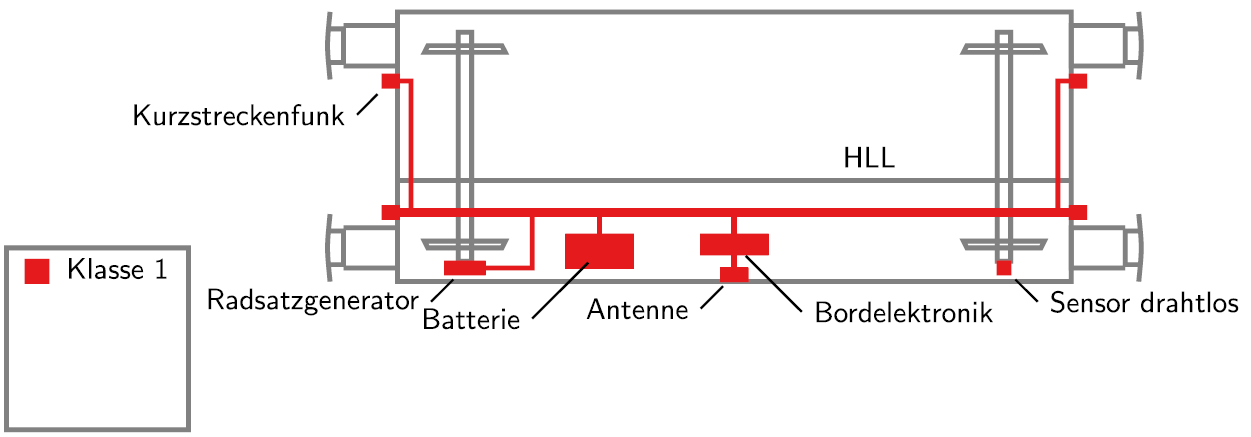
\includegraphics[width=\textwidth]{Bilder/Ausbaustufen_1.PNG}
    \caption{Klasse 1 mit Stromversorgung, Telematik und Datenvernetzung - angelehnt an \cite{ETR_3} }
    \label{fig:Klasse1}
\end{figure} 
In der ersten Ausbaustufe, siehe Abbildung \ref{fig:Klasse1}, ist die Anbringung einer Bordelektronik mit  entsprechender Spannungsversorgung geplant. Die Spannungsversorgung kann als Batterie mit Speisung durch einen Radsatzgenerator, Solarpanels oder ähnlichem realisiert werden oder auch als Pufferbatterie mit Speisung durch AK. Dazu kommen verschiedene Antennen und Kurzstreckenfunk zur Kommunikation mit anderen Wagen. Auch Sensoren zur Erfassung verschiedener Telematikfunktionen sind geplant.\par
In diesem Stadium ist der Wagen an sich noch nicht 'schlauer' als ein nicht ausgerüsteter Wagen, aber er kann sich mitteilen. Mitteilungen könne sein: Standort, Belandung, Laufleistung, (ungewöhnliche) Vibrationen (beispielsweise durch Falschstellen), Heißläuferdedektion, letzte Wartungsintervalle, Zustand der Bremse und vieles mehr.\par
\subsection{Ausbaustufe 2: Ausbaustufe 1 + Automatisierung der Bremsbedienung}
\begin{figure}[htbp] 
    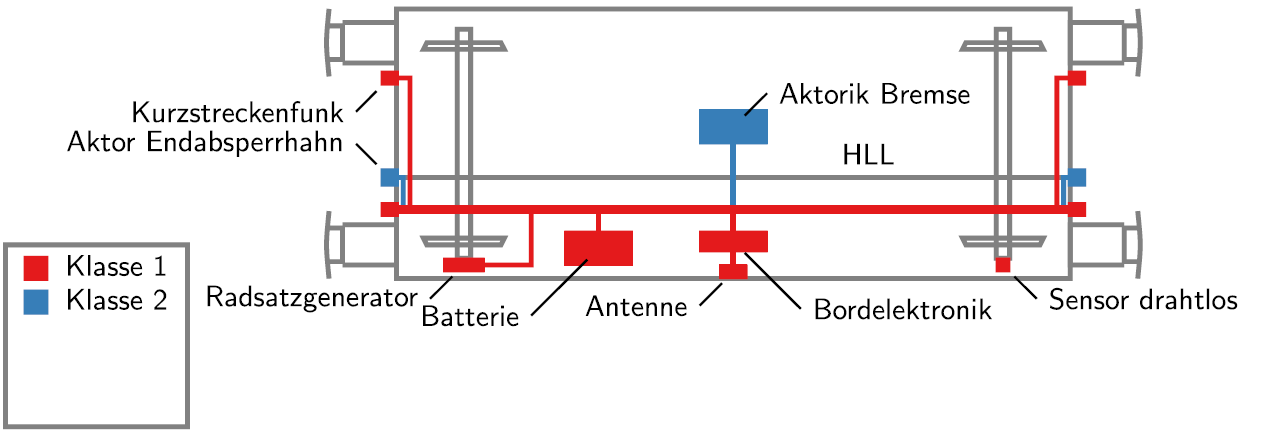
\includegraphics[width=\textwidth]{Bilder/Ausbaustufen_2.PNG}
    \caption{Klasse 2 bestehend aus Klasse 1 und der Automatisierung der Bremsbedienung - angelehnt an \cite{ETR_3}}
    \label{fig:Klasse2}
\end{figure} 
In der zweiten Ausbaustufe ist eine zusätzliche Aktorik für Endabsperrhähne und Handbremse geplant. Dadurch kann ein Teil der Bremsbedienung so weit automatisiert werden, dass ein Einstellen der Bremsart anhand von anderen Wagen im Wagenzug, Gewicht und Bremsfähigkeit möglich ist. Außerdem ist die automatische Parkbremse realisiert.\par
\subsection{Ausbaustufe 3: Ausbaustufe 2 + ep-''light''-Bremsen}
\begin{figure}[htbp] 
    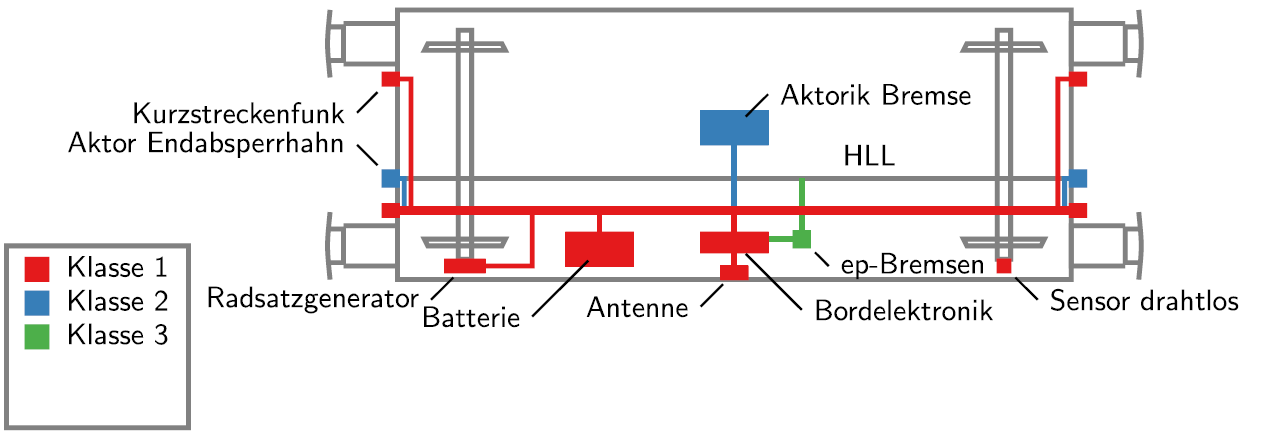
\includegraphics[width=\textwidth]{Bilder/Ausbaustufen_3.PNG}
    \caption{Klasse 3 bestehend aus Klasse 2 und der eingeführten ep-''light'-Bremse - angelehnt an \cite{ETR_3}}
    \label{fig:Klasse3}
\end{figure} 
In der dritten Ausbaustufe kommt zusätzlich zur Bremsbedienung auch die Ep-''light''-Bremse hinzu. Diese sorgt für eine für kürzere Bremswege und/oder höhere Geschwindigkeiten.\par
\subsection{Ausbaustufe 4: Ausbaustufe 3 + automatisierter Zugschluss}
\begin{figure}[htbp] 
    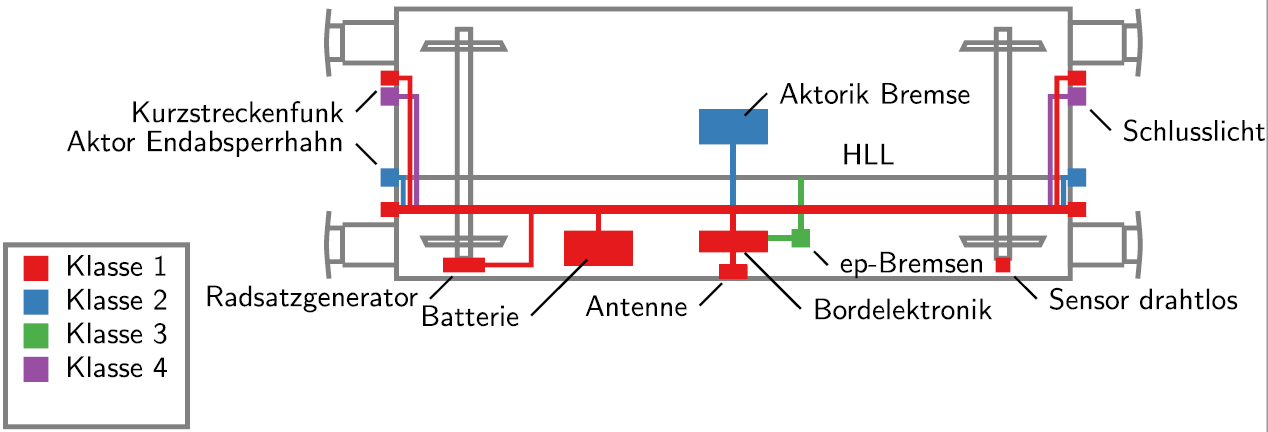
\includegraphics[width=\textwidth]{Bilder/Ausbaustufen_4.PNG}
    \caption{Klasse 4 bestehend aus Klasse 3 und der Automatisierung des Zugschlusses - angelehnt an \cite{ETR_3}}
    \label{fig:Klasse4}
\end{figure} 
In der vierten Ausbaustufe ist ein automatisierter Zugschluss geplant. Dieser soll das Anbringen des Zugschlusssignals am letzten Wagen ablösen. Dies wird eventuell vom Personal noch Manuell erledigt. Dau muss die Person den gesamten Zug von bis zu 700m ablaufen um die die entsprechenden Signale am letzten Wagen anzubringen. Das Zugschlusssignal hat außerdem die Funktion die Zugintigrität zu gewährleisten. 
\subsection{Ausbaustufe 5: Ausbaustufe 4 + Rangierantrieb}
\begin{figure}[htbp] 
    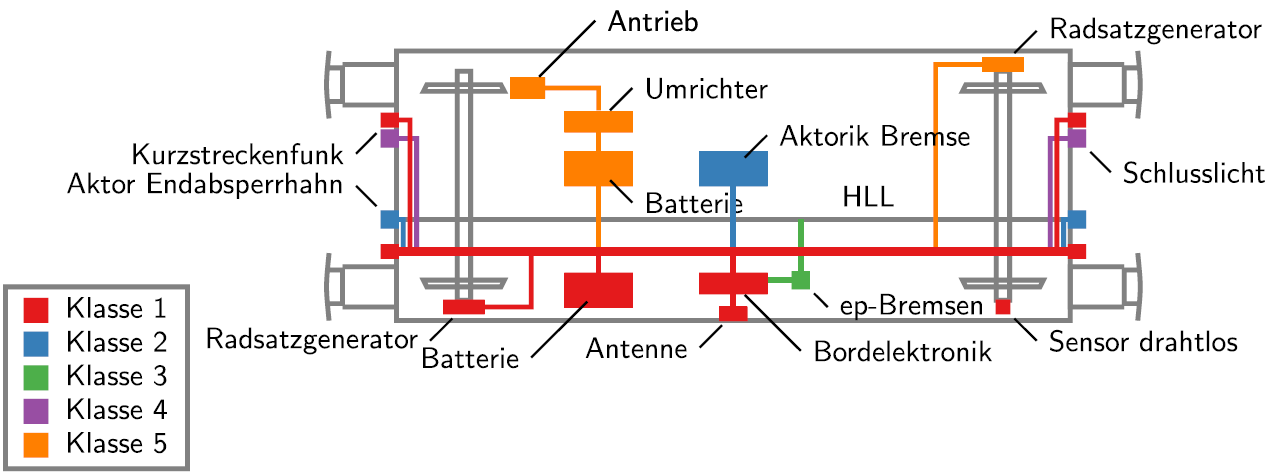
\includegraphics[width=\textwidth]{Bilder/Ausbaustufen_5.PNG}
    \caption{Klasse 5 bestehend aus Klasse 4 und einem Rangierantrieb - angelehnt an \cite{ETR_3}}
    \label{fig:Klasse5}
\end{figure} 
In der fünften Ausbaustufe kommt der Rangierantrieb hinzu. Damit dieser ohne Probleme funktioniert brauch er neben einem Antrieb zusätzlich eine weitere Batterie und Umrichter. Zur Speisung der zweiten Batterie wird auch ein zweiter Radsatzgenerator benötigt.\par
In diesem Stadium kann von einem automatisierten Güterwagen gesprochen werden. Er kann selbstständig bei der ''Briefkastenbedienung'' assistieren und auf dem Werksgelände ohne Rangierlok verfahren.\par

 \newpage
    \section{Anforderungen}
\textbf{Einfügen: Wie lang sind Lösezeiten, Verwendung Handbremse, Umlegen Endabsperrhähne}\par
\textbf{Sicherheitsrelevanz, Bedienen, Beobachten, Anbringungspunkte von Bauteilen -- gefedert? -- Bahntauglichkeit}\par
\subsection{Allgemeine und nicht funktionale Anforderungen}














%\begin{feat}
%automatische Zugschlussanzeige
%\end{feat}
%\begin{feat}
%Rangierantrieb
%\end{feat}%\newpage
    \section{Fazit} \newpage
%Hauptteil Ende

%Anhang Beginn
\pagenumbering{Roman}
    \printbibliography[heading=bibintoc, title={Quellenverzeichnis}] \newpage
    \appendix
    %\section{Zugehörige Dokumente}
Hier folgt eine Auflistung an potentiell interessanten Dokumenten für das Verständnis des Lastenhefts.
\begin{dok}[RIL 915]
Bremsen im Betrieb bedienen und prüfen
\end{dok}
\begin{dok}[RIL 936]
Technische Wagenbehandlung im Betrieb (Güterwagen)
\end{dok}
\begin{dok}[AZAP]
Antrag  auf  Gewährung  einer  Bundeszuwendung  auf  Ausgabenbasis
\end{dok}\newpage
    \section{Bremsprobe}\newpage
    \section{RIL 936 - Technische Wagenbehandlung im Betrieb (Güterwagen) - Auszug}
Die Technischen Wagenbehandlungsarten stellen sicher,
dass die im Einsatz befindlichen Wagen betriebssicher
sind. Die Prüfung der Verkehrstauglichkeit ist besonders
geregelt.\par 
Die technische Wagenbehandlung darf nur durchgeführt
werden, wenn die Bedingungen des Arbeitsschutzes hergestellt
sind.\par
Die technischen Wagenbehandlungsarten werden in folgenden
Stufen ihrer Ausführung beschrieben.
\subsection{TWb Stufe 1: Behandlung vor einer Rangierfahrt}
\textbf{Ziel}\par
Durch die Behandlung der Stufe 1 soll der betriebssichere
Zustand der Wagen sowie deren Ladungen und intermodale
Ladeeinheiten (ILE) für die anschließende Rangierfahrt
festgestellt werden.\par
\textbf{Arbeitsumfang}\par
Die Behandlung der Stufe 1 beinhaltet eine Sichtprüfung
der Wagen, Ladungen und ILE auf Schäden und Mängel,
welche die Sicherheit der Rangierfahrt beeinträchtigen –
soweit sie vom Boden aus, neben dem Fahrzeug stehend,
erkennbar sind.\par
Dabei werden Wagen, Ladungen oder ILE nicht betreten
oder geöffnet.\par
Wagen, Ladungen und ILE werden in der Behandlungsstufe
1 augenscheinlich daraufhin geprüft, ob z.B.
\begin{itemize}
    \item die ordnungsgemäße Stellung von Türen, Schiebewände, Hauben, Dächer, Klappen, Sicherungsmittel usw. geschlossen und verriegelt sind, offensichtliche Schäden vorliegen, z. B. durch die Be- oder Entladung bzw.
    \item Eingriffe oder Manipulationen vorliegen,
    \item Tritte, Griffe, Handläufe und Aufstiegsleitern in bestimmungsgemäßem Zustand sind,
    \item kein Ladegut austritt,
    \item lose Wagenbestandteile ordnungsgemäß festgelegt oder befestigt sind,
    \item keine losen Gegenstände auf dem Wagen liegen, die die Betriebssicherheit gefährden können und
    \item Ladungssicherungen nicht beschädigt sind.
\end{itemize}
\textbf{Einzuleitende Maßnahmen und Dokumentation}\par
Bei erkannten Schäden und Mängeln sind Maßnahmen wie
\begin{itemize}
    \item Schaden oder Mangel selbst beheben (z.B. Tür schließen).
    \item Wagen von der Rangierfahrt ausschließen
\end{itemize}
einzuleiten.\par
Können vorgefundene Schäden/ Mängel nicht behoben
werden, sind erforderliche Maßnahmen über die zuständige
Dispostelle einzuleiten.
\subsection{TWb Stufe 2: Prüfung nach Abstellung (PnA}
\textbf{Ziel}\par
Durch die Behandlung der Stufe 2 sollen Einwirkungen Dritter während der Abstellzeit des Zuges (Wagen, Ladungen und ILE) festgestellt bzw. behoben werden, um für die anschließende Zugfahrt (inkl. Feststellen der Fahrbereitschaft) den sicheren Betrieb zu gewährleisten.\par
\textbf{Arbeitsumfang}\par
Die Behandlung Stufe 2 beinhaltet zur Feststellung der
Abfahrbereitschaft eine beidseitige Sichtprüfung der Wagen,
Ladungen und ILE. \par
Wagen, Ladungen und ILE werden augenscheinlich auf offensichtliche
Eingriffe oder Manipulationen geprüft.\par
Bei dieser augenscheinlichen Behandlung ist besonders
darauf zu achten, dass z.B.
\begin{itemize}
    \item Türen, Seitenwände, Dächer und Hauben usw. am Fahrzeug geschlossen und verriegelt sind,
    \item lose/bewegliche Fahrzeugteile festgelegt sind,
    \item Fahrzeuge ordnungsgemäß gekuppelt sind,
    \item Ladungssicherungen nicht beschädigt oder offensichtlich entfernt sind und
    \item dass kein Ladegut austritt.
\end{itemize}
Bei der Behandlung der Stufe 2 muss der Abgleich der ersten und letzten Wagennummer (Wagenliste oder Bremszettel) durchgeführt werden.\par
\textbf{Einzuleitende Maßnahmen und Dokumentation}\par
Bei erkannten Schäden und Mängel sind Abhilfemaßnahmen wie
\begin{itemize}
    \item Schaden oder Mangel selbst beheben (z.B. Tür schließen)
    \item Wagen von der Zugfahrt ausschließen einzuleiten.
\end{itemize}
Festgestellte Schäden und Mängeln sind mit Schadzettel (z.B. Störmeldezettel Tf) zu dokumentieren und dem zuständigen Disponenten zu melden. Können Sie deren Auswirkungen nicht sicher abschätzen oder nicht beheben, ist die weitere Vorgehensweise mit dem zuständigen Disponenten festzulegen.\par
Vor dem Einleiten von Abhilfemaßnahmen nach offensichtlichen Eingriffen oder von Manipulationen an Wagen wie z.B. geöffnete Türen/Verschlüsse oder das Anbringen
von nicht identifizierbaren Gegenständen, ist die weitere Vorgehensweise unverzüglich mit der zuständigen Dispostelle abzustimmen. Weitere Maßnahmen könnten von dem Ergebnis der Spurensicherung durch die Polizeibehörden abhängig sein. \par
Hinweise auf Schäden und Mängel sowie weiterführende Regelungen und Maßnahmen, sind im „Kriterienkatalog für Schäden und Mängel“ der Ril 936ff geregelt.\par
\subsection{TWb Stufe 3: Prüfung vor der Zugfahrt}
\textbf{Ziel} \par
Feststellung des betriebssicheren Zustands der Wagen,
Ladungen und ILE vor der Zugfahrt.\par
\textbf{Varianten} \par
Für die Stufe 3 können verschiedene Varianten erforderlich sein:
\begin{itemize}
    \item Behandlung vor der Zugfahrt - DBCDE Verkehr
    \item Behandlung vor der Zugfahrt – AVV Verkehr
\end{itemize}
\textbf{Besonderheiten} \par
Sendungen, an deren Transport besondere Bedingungen gestellt sind (z.B. außergewöhnliche Sendungen, Militärverkehr (MV) usw.) bedürfen einer vorherigen Wagensonderuntersuchung
(WSU) im Rahmen der Stufe 4 mit Abnahme. Die Dokumentation ist nach Ril 936.0301 vorzunehmen.\par
\textbf{Arbeitsumfang} \par
Die Durchführung der Stufe 3 erfolgt i.d.R. am fertig gebildeten Zug/ Zugteil. Dabei werden Systemdaten grundsätzlich mittels vorhandener mobiler DV überprüft und dokumentiert. Grundsätzlich ist die Durchführung der Stufe 3 mit der Reihung zu verbinden.\par
Die Stufe 3 beinhaltet die Feststellung
\begin{itemize}
    \item des betriebssicheren Zustandes der Fahrzeuge und Ladungen,
    \item das Ladungen und deren Sicherung soweit einsehbar, nicht beschädigt sind,
    \item auf Überladung,
    \item der Einhaltung bestimmter Zugbildungskriterien wie z.B.
    \begin{itemize}
        \item Kuppelzustand allgemein (gekuppelt und geschlaucht),
        \item Prüfung auf das Einstellen nicht zugelassener Wagen (z.B. schwerbeschädigte Wagen),
        \item Prüfung auf außergewöhnliche Sendungen (Stellung im Zug, Schutzabstände),
        \item Prüfung der Schutzabstände bei Gefahrgutsendungen GGVSEB,
        \item Abgleich der Ladungsgewichte sowie Wagenreihungskontrolle.
    \end{itemize}
\end{itemize}
\textbf{Einzuleitende Maßnahmen und Dokumentation} \par
Bei erkannten Schäden und Mängeln sind Abhilfemaßnahmen wie
\begin{itemize}
    \item Schaden oder Mangel selbst beheben (z.B. Tür schließen),
    \item Wagen von der Zugfahrt ausschließen
\end{itemize}
einzuleiten.\par
Festgestellte Schäden und Mängel sind mit dem erforderlichen Schadzettel zu bezetteln, zu dokumentieren und soweit erforderlich dem zuständigen Disponenten zu melden. Können Sie deren Auswirkungen nicht sicher abschätzen oder nicht beheben, ist die weitere Vorgehensweise mit dem zuständigen Disponenten festzulegen.\par
Hinweise auf Schäden und Mängel sowie weiterführende Regelungen und Maßnahmen, sind im „Kriterienkatalog für Schäden und Mängel“ der Ril 936ff geregelt.
\subsection{TWb Stufe 4: Untersuchung und Qualitätscheck Wagen}
\textbf{Ziel} \par
Die Feststellung des betriebssicheren Zustands der Wagen,
Ladungen und ILE.
\begin{itemize}
    \item Beurteilung von Schäden und Mängel und ausführliche Dokumentation,
    \item Prüfung auf uneingeschränkte Nutzbarkeit bzw. Festlegung der weiteren Einsatzkriterien und ausführliche Dokumentation
    \item Abhilfe durch Kleinstschadenbeseitigung oder Behandlung zum Verbleib im Betrieb.
    \item Erfassung und Beschreibung von Schäden zur Arbeitsvorbereitung für die Instandhaltung und Entscheidungsfindung für den Halter.
\end{itemize}
\textbf{Varianten} \par
Für die Stufe 4 können verschiedene Untersuchungen erforderlich sein:
\begin{itemize}
    \item Untersuchung von Wagen am Zug oder Zugteil
    \item Untersuchung von leeren Wagen vor der Beladung am Zug oder Zugteil im kombinierten Verkehr (siehe Ril 936.0103 KV)
    \item Untersuchung von beladenen Wagen am Zug oder Zugteil im Militärverkehr (siehe Ril 936.0104 MV)
\end{itemize}
Für die Durchführung der WSU ist, soweit diese Tätigkeiten nicht im Zeitfenster der Behandlungsart durchgeführt werden können, eine besondere Beauftragung nach Ril 936.0301 (Vordruck 936.0301V32) erforderlich.\par
\textbf{Besonderheiten} \par
Wird eine Untersuchung der Stufe 4 durchgeführt, ersetzt diese die Stufe 1, 2, 3, 3 KV und 3 AVV in jedem Fall. \par
\textbf{Arbeitsumfang} \par
Die Durchführung der Stufe 4 erfolgt i.d.R.am fertig gebildeten Zug/ Zugteil. Dabei werden Systemdaten grundsätzlich mittels vorhandener mobiler DV überprüft und dokumentiert. Grundsätzlich ist die Durchführung der Stufe 4 mit der Reihung zu verbinden. Weiter sind erforderliche Beschädigungs- und Mängelberichte zu erstellen.\par
Die Stufe 4 beinhaltet die Feststellung
\begin{itemize}
    \item des betriebssicheren Zustandes der Fahrzeuge und Ladungen,
    \item das Ladungen und deren Sicherung soweit einsehbar, nicht beschädigt sind,
    \item auf Überladung
    \item bestimmter Zugbildungskriterien wie z.B.
    \begin{itemize}
        \item Kuppelzustand allgemein (gekuppelt und geschlaucht),
        \item Prüfung auf das Einstellen nicht zugelassener Wagen (z.B. schwerbeschädigte Wagen),
        \item Prüfung auf außergewöhnliche Sendungen (Stellung im Zug, Schutzabstände),
        \item Prüfung der Schutzabstände bei Gefahrgutsendungen GGVSEB,
        \item Abgleich der Ladungsgewichte sowie Wagenreihungskontrolle.
    \end{itemize}
\end{itemize}
Die Suche nach verdeckten oder schwer erkennbaren Schäden und Mängeln muss erfolgen, wenn Merkmale an den Bauteilen, die Lage der Bauteile zueinander, Funktionsstörungen oder andere Gründe auf das Vorliegen von Unregelmäßigkeiten schließen lassen. Das dabei erforderliche Messen und Berechnen einzelner Maße ist unter Verwendung von Hilfs- und Messmitteln durchzuführen.\par
\textbf{Einzuleitende Maßnahmen und Dokumentation} \par
Bei erkannten Schäden und Mängeln sind Abhilfemaßnahmen wie
\begin{itemize}
    \item Schaden oder Mangel selbst beheben (siehe Ril 936.13 bzw. 936.95),
    \item Wagen von der Zugfahrt ausschließen
\end{itemize}
einzuleiten.




%Anhang Ende

\end{document}